         \chapter{Statistics}
    \setcounter{figure}{1}
    \setcounter{subfigure}{1}
    \label{ea5128681e667fecbf404a0996287edc}
%          \section{ Introduction and recap}
%     \nopagebreak
%             \label{m39403} $ \hspace{-5pt}\begin{array}{cccccccccccc}   
\includegraphics[width=0.75cm]{col11306.imgs/summary_fullmarks.png} &   \end{array} $ \hspace{2 pt}\raisebox{-5 pt}{} {(section shortcode: MG10114 )} \par 
%     
%     
%     \label{m39403*cid2}
% %             \subsection{ Introduction}
% %             \nopagebreak
%             
%       
      \label{m39403*id199946}Information in the form of numbers, graphs and tables is all around us; on television, on the radio or in the newspaper. We are exposed to crime rates, sports results, rainfall, government spending, rate of HIV/AIDS infection, population growth and economic growth.\par 
      \label{m39403*eip-765}This chapter demonstrates how Mathematics can be used to manipulate data, to represent or misrepresent trends and patterns and to provide solutions that are directly applicable to the world around us.
\par \label{m39403*id199957}Skills relating to the collection, organisation, display, analysis and interpretation of information that were introduced in earlier grades are developed further.\par 
%     \label{m39403*cid3}
%             \section{ Recap of Earlier Work}
%             \nopagebreak
%             
%       
        \label{m39403*uid1}
            \section{ Data and Data Collection}
            \nopagebreak
         \label{m39403*id200309}The collection of data has been introduced in earlier grades as a method of obtaining answers to questions about the world around us. This work will be briefly reviewed.\par 
%         \label{m39403*uid2}
%             \subsubsection{ Data}
%             \nopagebreak
%             
%           
\par
            \label{m39403*fhsst!!!underscore!!!id85}\begin{definition}
	  \begin{tabular*}{15 cm}{m{15 mm}m{}}
	\hspace*{-50pt}  
\includegraphics[width=0.5in]{col11306.imgs/psflag2.png}   & \Definition{   \label{id2616525}\textbf{ Data }} { \label{m39403*meaningfhsst!!!underscore!!!id85}
          \label{m39403*id200337}Data refers to the pieces of information that have been observed and recorded, from an experiment or a survey. There are two types of data: primary and secondary. The word "data" is the plural of the word "datum", and therefore one should say, "the data are" and not "the data is". \par 
           } 
      \end{tabular*}
      \end{definition}
          \label{m39403*id200350}Data can be classified as \textit{primary} or \textit{secondary}, and primary or secondary data can be classified as \textit{qualitative} or \textit{quantitative}. Figure~16.1 summarises the classifications of data.\par 
    \setcounter{subfigure}{0}
	\begin{figure}[H] % horizontal\label{m39403*uid3}
    \begin{center}
    \rule[.1in]{\figurerulewidth}{.005in} \\
        \label{m39403*uid3!!!underscore!!!media}\label{m39403*uid3!!!underscore!!!printimage}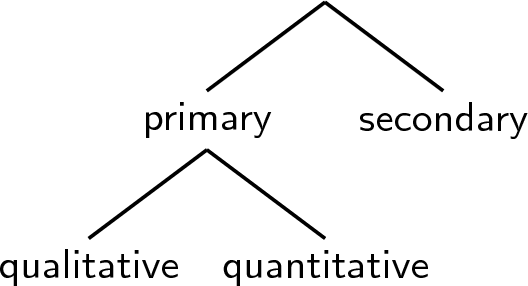
\includegraphics[width=300px]{col11306.imgs/m39403_MG10C16_001.png} % m39403;MG10C16\_001.png;;;6.0;8.5;
      \vspace{2pt}
    \vspace{\rubberspace}\par \begin{cnxcaption}
	  \small \textbf{Figure 16.1: }Classes of data.
	\end{cnxcaption}
    \vspace{.1in}
    \rule[.1in]{\figurerulewidth}{.005in} \\
    \end{center}
 \end{figure}       
          \label{m39403*id200390}\begin{description}[noitemsep]
            \label{m39403*uid4}
            \item[Primary data:]
          describes the original data that have been collected. This type of data is also known as \textit{raw} data. Often the primary data set is very large and is therefore summarised or processed to extract meaningful information.
\label{m39403*uid5}
            \item[Qualitative data:]
          is information that cannot be written as numbers, for example, if you were collecting data from people on how they feel or what their favourite colour is.
\label{m39403*uid6}
            \item[Quantitative data:]
          is information that can be written as numbers, for example, if you were collecting data from people on their height or weight.
\label{m39403*uid7}
            \item[Secondary data:]
          is primary data that has been summarised or processed, for example, the set of colours that people gave as favourite colours would be secondary data because it is a summary of responses.
\end{itemize}
          \label{m39403*id200459}Transforming primary data into secondary data through analysis, grouping or organisation into secondary data is the process of generating information.\par 
        \label{m39403*uid8}
            \subsubsection{ Purpose of Collecting Primary Data}
            \nopagebreak
          \label{m39403*id200473}Data is collected to provide answers that help with understanding a particular situation. Here are examples to illustrate some real world data collections scenarios in the categories of qualitative and quantitative data.\par 
        \label{m39403*id200480}
            \subsubsection{ Qualitative Data}
            \nopagebreak
          \label{m39403*id200486}\begin{itemize}[noitemsep]
            \label{m39403*uid9}\item The local government might want to know how many residents have electricity and might ask the question: "Does your home have a safe, independent supply of electricity?"
\label{m39403*uid10}\item A supermarket manager might ask the question: ``What flavours of soft drink should be stocked in my supermarket?" The question asked of customers might be ``What is your favourite soft drink?'' Based on the customers' responses (i.e. which flavours are chosen), the manager can make an informed decision as to what soft drinks to stock.
\label{m39403*uid11}\item A company manufacturing medicines might ask ``How effective is our pill at relieving a headache?'' The question asked of people using the pill for a headache might be: ``Does taking the pill relieve your headache?'' Based on responses, the company learns how effective their product is.
\label{m39403*uid12}\item A motor car company might want to improve their customer service, and might ask their customers: ``How can we improve our customer service?''
\end{itemize}
        \label{m39403*id200551}
            \subsubsection{ Quantitative Data}
            \nopagebreak
          \label{m39403*id200557}\begin{itemize}[noitemsep]
            \label{m39403*uid13}\item A cell phone manufacturing company might collect data about how often people buy new cell phones and what factors affect their choice, so that the cell phone company can focus on those features that would make their product more attractive to buyers.
\label{m39403*uid14}\item A town councillor might want to know how many accidents have occurred at a particular intersection, to decide whether a robot should be installed. The councillor would visit the local police station to research their records to collect the appropriate data.
\label{m39403*uid15}\item A supermarket manager might ask the question: ``What flavours of soft drink should be stocked in my supermarket?" The question asked of customers might be ``What is your favourite soft drink?'' Based on the customers' responses (i.e. the number of customers who liked soft drink A), the manager can make an informed decision as to what soft drinks to stock. 
\end{itemize}
          \label{m39403*id200605}However, it is important to note that different questions reveal different features of a situation, and that this affects the ability to understand
the situation. For example, if the first question in the list was re-phrased to be: "Does your home have electricity?" then if you answered yes, but you were getting your electricity from a neighbour, then this would give the wrong impression that you did not need an independent supply of electricity.\par 
      \label{m39403*uid16}
            \subsubsection{ Methods of Data Collection}
            \nopagebreak
        \label{m39403*id200621}The method of collecting the data must be appropriate to the question being asked. Some examples of data collecting methods are:\par 
        \label{m39403*id200626}\begin{enumerate}[noitemsep, label=\textbf{\arabic*}. ] 
            \label{m39403*uid17}\item Questionnaires, surveys and interviews
\label{m39403*uid18}\item Experiments
\label{m39403*uid19}\item Other sources (friends, family, newspapers, books, magazines and the Internet)
\end{enumerate}
        \label{m39403*id200664}The most important aspect of each method of data collecting is to clearly formulate the question that is to be answered. The details of the data collection should therefore be structured to take your question into account.\par 
        \label{m39403*id200670}For example, questionnaires, interviews or surveys would be most appropriate for the list of questions in "Purpose of Collecting Primary Data" (Section~16.1.2.1.2: Purpose of Collecting Primary Data).\par 
      \label{m39403*uid20}
            \subsubsection{ Samples and Populations}
            \nopagebreak
        \label{m39403*id200688}Before the data collecting starts, it is important to decide how much data is needed to make sure that the results give an accurate reflection to the required answers. Ideally, the study should be designed to maximise the amount of information collected while minimising the effort. The concepts of \textit{populations} and \textit{samples} is vital to minimising effort.\par 
        \label{m39403*id200705}The following terms should be familiar:\par 
        \label{m39403*id200708}\begin{description}[noitemsep]
            \label{m39403*uid21}
            \item[Population:]
          describes the entire group under consideration in a study. For example, if you wanted to know how many learners in your school got the flu each winter, then your population would be all the learners in your school.
\label{m39403*uid22}
            \item[Sample:]
          describes a group chosen to represent the population under consideration in a study. For example, for the survey on winter flu, you might select a sample of learners, maybe one from each class.
\label{m39403*uid23}
            \item[Random sample:]
          describes a sample chosen from a population in such a way that each member of the population has an equal chance of being chosen.
\end{itemize}
        \label{m39403*id200757}
    \setcounter{subfigure}{0}
	\begin{figure}[H] % horizontal\label{m39403*id200760}
    \begin{center}
    \label{m39403*id200760!!!underscore!!!media}\label{m39403*id200760!!!underscore!!!printimage}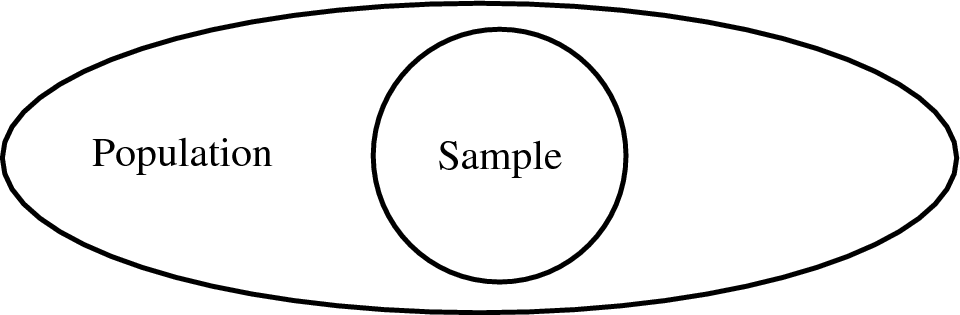
\includegraphics[width=300px]{col11306.imgs/m39403_MG10C16_002.png} % m39403;MG10C16\_002.png;;;6.0;8.5;
      \vspace{2pt}
    \vspace{.1in}
    \end{center}
 \end{figure}       
        \par 
        \label{m39403*id200766}Choosing a representative sample is crucial to obtaining results that are unbiased. For example, if we wanted to determine whether peer pressure affects the decision to start smoking, then the results would be different if only boys were interviewed, compared to if only girls were interviewed, compared to both boys and girls being interviewed.\par 
        \label{m39403*id200773}Therefore questions like: "How many interviews are needed?" and "How do I select the candidates for the interviews?" must be asked during the design stage of the sampling process.\par 
        \label{m39403*id200777}The most accurate results are obtained if the entire population is sampled for the survey, but this is expensive and time-consuming. The next best method is to \textit{randomly} select a sample of subjects for the interviews. This means that whatever the method used to select subjects for the interviews, each subject has an equal chance of being selected. There are various methods of doing this for example, names can be picked out of a hat or can be selected by using a random number generator. Most modern scientific calculators have a random number generator or you can find one on a spreadsheet program on a computer.\par 
        \label{m39403*id200791}So, if you had a total population of 1 000 learners in your school and you randomly selected 100, then that would be the sample that is used to conduct your survey.\par 
    \label{m39403*cid4}
            \subsection{ Example Data Sets}
            \nopagebreak
      \label{m39403*id200805}The remainder of this chapter deals with the mathematical details that are required to analyse the data collected.\par 
      \label{m39403*id200809}The following are some example sets of data which can be used to apply the methods that are being explained.\par 
      \label{m39403*uid24}
            \subsubsection{ Data Set 1: Tossing a Coin}
            \nopagebreak
        \label{m39403*id200822}A fair coin was tossed 100 times and the values on the top face were recorded. The data are recorded in "Data Set 1: Tossing a coin" (Table 16.1).\par 
    % \textbf{m39403*uid25}\par
          \begin{table}[H]
    % \begin{table}[H]
    % \\ '' '0'
        \begin{center}
      \label{m39403*uid25}
    \noindent
    \tabletail{%
        \hline
        \multicolumn{10}{|p{\mytableboxwidth}|}{\raggedleft \small \sl continued on next page}\\
        \hline
      }
      \tablelasttail{}
      \begin{xtabular}[t]{|l|l|l|l|l|l|l|l|l|l|}\hline
        H &
        T &
        T &
        H &
        H &
        T &
        H &
        H &
        H &
        H% make-rowspan-placeholders
     \tabularnewline\cline{1-1}\cline{2-2}\cline{3-3}\cline{4-4}\cline{5-5}\cline{6-6}\cline{7-7}\cline{8-8}\cline{9-9}\cline{10-10}
      %--------------------------------------------------------------------
        H &
        H &
        H &
        H &
        T &
        H &
        H &
        T &
        T &
        T% make-rowspan-placeholders
     \tabularnewline\cline{1-1}\cline{2-2}\cline{3-3}\cline{4-4}\cline{5-5}\cline{6-6}\cline{7-7}\cline{8-8}\cline{9-9}\cline{10-10}
      %--------------------------------------------------------------------
        T &
        T &
        H &
        T &
        T &
        H &
        T &
        H &
        T &
        H% make-rowspan-placeholders
     \tabularnewline\cline{1-1}\cline{2-2}\cline{3-3}\cline{4-4}\cline{5-5}\cline{6-6}\cline{7-7}\cline{8-8}\cline{9-9}\cline{10-10}
      %--------------------------------------------------------------------
        H &
        H &
        T &
        T &
        H &
        T &
        T &
        H &
        T &
        T% make-rowspan-placeholders
     \tabularnewline\cline{1-1}\cline{2-2}\cline{3-3}\cline{4-4}\cline{5-5}\cline{6-6}\cline{7-7}\cline{8-8}\cline{9-9}\cline{10-10}
      %--------------------------------------------------------------------
        T &
        H &
        H &
        H &
        T &
        T &
        H &
        T &
        T &
        H% make-rowspan-placeholders
     \tabularnewline\cline{1-1}\cline{2-2}\cline{3-3}\cline{4-4}\cline{5-5}\cline{6-6}\cline{7-7}\cline{8-8}\cline{9-9}\cline{10-10}
      %--------------------------------------------------------------------
        H &
        T &
        T &
        T &
        T &
        H &
        T &
        T &
        H &
        H% make-rowspan-placeholders
     \tabularnewline\cline{1-1}\cline{2-2}\cline{3-3}\cline{4-4}\cline{5-5}\cline{6-6}\cline{7-7}\cline{8-8}\cline{9-9}\cline{10-10}
      %--------------------------------------------------------------------
        T &
        T &
        H &
        T &
        T &
        H &
        T &
        T &
        H &
        T% make-rowspan-placeholders
     \tabularnewline\cline{1-1}\cline{2-2}\cline{3-3}\cline{4-4}\cline{5-5}\cline{6-6}\cline{7-7}\cline{8-8}\cline{9-9}\cline{10-10}
      %--------------------------------------------------------------------
        H &
        T &
        T &
        H &
        T &
        T &
        T &
        T &
        H &
        T% make-rowspan-placeholders
     \tabularnewline\cline{1-1}\cline{2-2}\cline{3-3}\cline{4-4}\cline{5-5}\cline{6-6}\cline{7-7}\cline{8-8}\cline{9-9}\cline{10-10}
      %--------------------------------------------------------------------
        T &
        H &
        T &
        T &
        H &
        H &
        H &
        T &
        H &
        T% make-rowspan-placeholders
     \tabularnewline\cline{1-1}\cline{2-2}\cline{3-3}\cline{4-4}\cline{5-5}\cline{6-6}\cline{7-7}\cline{8-8}\cline{9-9}\cline{10-10}
      %--------------------------------------------------------------------
        T &
        T &
        T &
        H &
        H &
        T &
        T &
        T &
        H &
        T% make-rowspan-placeholders
     \tabularnewline\cline{1-1}\cline{2-2}\cline{3-3}\cline{4-4}\cline{5-5}\cline{6-6}\cline{7-7}\cline{8-8}\cline{9-9}\cline{10-10}
      %--------------------------------------------------------------------
    \end{xtabular}
      \end{center}
    \begin{center}{\small\bfseries Table 16.1}: Results of 100 tosses of a fair coin. H means that the coin landed heads-up and T means that the coin landed tails-up.\end{center}
    \begin{caption}{\small\bfseries Table 16.1}: Results of 100 tosses of a fair coin. H means that the coin landed heads-up and T means that the coin landed tails-up.\end{caption}
\end{table}
    \par
      \label{m39403*uid26}
            \subsubsection{ Data Set 2: Casting a die}
            \nopagebreak
        \label{m39403*id201632}A fair die was cast 100 times and the values on the top face were recorded. The data are recorded in "Data Set 2: Casting a die" (Section~16.1.3.2: Data Set 2: Casting a die).\par 
    % \textbf{m39403*uid27}\par
          \begin{table}[H]
    % \begin{table}[H]
    % \\ '' '0'
        \begin{center}
      \label{m39403*uid27}
    \noindent
    \tabletail{%
        \hline
        \multicolumn{20}{|p{\mytableboxwidth}|}{\raggedleft \small \sl continued on next page}\\
        \hline
      }
      \tablelasttail{}
      \begin{xtabular}[t]{|l|l|l|l|l|l|l|l|l|l|l|l|l|l|l|l|l|l|l|l|}\hline
        3 &
        5 &
        3 &
        6 &
        2 &
        6 &
        6 &
        5 &
        5 &
        6 &
        6 &
        4 &
        2 &
        1 &
        5 &
        3 &
        2 &
        4 &
        5 &
        4% make-rowspan-placeholders
     \tabularnewline\cline{1-1}\cline{2-2}\cline{3-3}\cline{4-4}\cline{5-5}\cline{6-6}\cline{7-7}\cline{8-8}\cline{9-9}\cline{10-10}\cline{11-11}\cline{12-12}\cline{13-13}\cline{14-14}\cline{15-15}\cline{16-16}\cline{17-17}\cline{18-18}\cline{19-19}\cline{20-20}
      %--------------------------------------------------------------------
        1 &
        4 &
        3 &
        2 &
        6 &
        6 &
        4 &
        6 &
        2 &
        6 &
        5 &
        1 &
        5 &
        1 &
        2 &
        4 &
        4 &
        2 &
        4 &
        4% make-rowspan-placeholders
     \tabularnewline\cline{1-1}\cline{2-2}\cline{3-3}\cline{4-4}\cline{5-5}\cline{6-6}\cline{7-7}\cline{8-8}\cline{9-9}\cline{10-10}\cline{11-11}\cline{12-12}\cline{13-13}\cline{14-14}\cline{15-15}\cline{16-16}\cline{17-17}\cline{18-18}\cline{19-19}\cline{20-20}
      %--------------------------------------------------------------------
        4 &
        2 &
        6 &
        4 &
        5 &
        4 &
        3 &
        5 &
        5 &
        4 &
        6 &
        1 &
        1 &
        4 &
        6 &
        6 &
        4 &
        5 &
        3 &
        5% make-rowspan-placeholders
     \tabularnewline\cline{1-1}\cline{2-2}\cline{3-3}\cline{4-4}\cline{5-5}\cline{6-6}\cline{7-7}\cline{8-8}\cline{9-9}\cline{10-10}\cline{11-11}\cline{12-12}\cline{13-13}\cline{14-14}\cline{15-15}\cline{16-16}\cline{17-17}\cline{18-18}\cline{19-19}\cline{20-20}
      %--------------------------------------------------------------------
        2 &
        6 &
        3 &
        2 &
        4 &
        5 &
        3 &
        2 &
        2 &
        6 &
        3 &
        4 &
        3 &
        2 &
        6 &
        4 &
        5 &
        2 &
        1 &
        5% make-rowspan-placeholders
     \tabularnewline\cline{1-1}\cline{2-2}\cline{3-3}\cline{4-4}\cline{5-5}\cline{6-6}\cline{7-7}\cline{8-8}\cline{9-9}\cline{10-10}\cline{11-11}\cline{12-12}\cline{13-13}\cline{14-14}\cline{15-15}\cline{16-16}\cline{17-17}\cline{18-18}\cline{19-19}\cline{20-20}
      %--------------------------------------------------------------------
        5 &
        4 &
        1 &
        3 &
        1 &
        3 &
        5 &
        1 &
        3 &
        6 &
        5 &
        3 &
        4 &
        3 &
        4 &
        5 &
        1 &
        2 &
        1 &
        2% make-rowspan-placeholders
     \tabularnewline\cline{1-1}\cline{2-2}\cline{3-3}\cline{4-4}\cline{5-5}\cline{6-6}\cline{7-7}\cline{8-8}\cline{9-9}\cline{10-10}\cline{11-11}\cline{12-12}\cline{13-13}\cline{14-14}\cline{15-15}\cline{16-16}\cline{17-17}\cline{18-18}\cline{19-19}\cline{20-20}
      %--------------------------------------------------------------------
        1 &
        3 &
        2 &
        3 &
        6 &
        3 &
        1 &
        6 &
        3 &
        6 &
        6 &
        1 &
        4 &
        5 &
        2 &
        2 &
        6 &
        3 &
        5 &
        3% make-rowspan-placeholders
     \tabularnewline\cline{1-1}\cline{2-2}\cline{3-3}\cline{4-4}\cline{5-5}\cline{6-6}\cline{7-7}\cline{8-8}\cline{9-9}\cline{10-10}\cline{11-11}\cline{12-12}\cline{13-13}\cline{14-14}\cline{15-15}\cline{16-16}\cline{17-17}\cline{18-18}\cline{19-19}\cline{20-20}
      %--------------------------------------------------------------------
        1 &
        1 &
        6 &
        4 &
        5 &
        1 &
        6 &
        5 &
        3 &
        2 &
        6 &
        2 &
        3 &
        2 &
        5 &
        6 &
        3 &
        5 &
        5 &
        6% make-rowspan-placeholders
     \tabularnewline\cline{1-1}\cline{2-2}\cline{3-3}\cline{4-4}\cline{5-5}\cline{6-6}\cline{7-7}\cline{8-8}\cline{9-9}\cline{10-10}\cline{11-11}\cline{12-12}\cline{13-13}\cline{14-14}\cline{15-15}\cline{16-16}\cline{17-17}\cline{18-18}\cline{19-19}\cline{20-20}
      %--------------------------------------------------------------------
        2 &
        6 &
        6 &
        3 &
        5 &
        4 &
        1 &
        4 &
        5 &
        1 &
        4 &
        1 &
        3 &
        4 &
        3 &
        6 &
        2 &
        4 &
        3 &
        6% make-rowspan-placeholders
     \tabularnewline\cline{1-1}\cline{2-2}\cline{3-3}\cline{4-4}\cline{5-5}\cline{6-6}\cline{7-7}\cline{8-8}\cline{9-9}\cline{10-10}\cline{11-11}\cline{12-12}\cline{13-13}\cline{14-14}\cline{15-15}\cline{16-16}\cline{17-17}\cline{18-18}\cline{19-19}\cline{20-20}
      %--------------------------------------------------------------------
        6 &
        1 &
        1 &
        2 &
        4 &
        5 &
        2 &
        5 &
        3 &
        4 &
        3 &
        4 &
        5 &
        3 &
        3 &
        3 &
        1 &
        1 &
        4 &
        3% make-rowspan-placeholders
     \tabularnewline\cline{1-1}\cline{2-2}\cline{3-3}\cline{4-4}\cline{5-5}\cline{6-6}\cline{7-7}\cline{8-8}\cline{9-9}\cline{10-10}\cline{11-11}\cline{12-12}\cline{13-13}\cline{14-14}\cline{15-15}\cline{16-16}\cline{17-17}\cline{18-18}\cline{19-19}\cline{20-20}
      %--------------------------------------------------------------------
        5 &
        2 &
        1 &
        4 &
        2 &
        5 &
        2 &
        2 &
        1 &
        5 &
        4 &
        5 &
        1 &
        5 &
        3 &
        2 &
        2 &
        5 &
        1 &
        1% make-rowspan-placeholders
     \tabularnewline\cline{1-1}\cline{2-2}\cline{3-3}\cline{4-4}\cline{5-5}\cline{6-6}\cline{7-7}\cline{8-8}\cline{9-9}\cline{10-10}\cline{11-11}\cline{12-12}\cline{13-13}\cline{14-14}\cline{15-15}\cline{16-16}\cline{17-17}\cline{18-18}\cline{19-19}\cline{20-20}
      %--------------------------------------------------------------------
    \end{xtabular}
      \end{center}
    \begin{center}{\small\bfseries Table 16.2}: Results of 200 casts of a fair die.\end{center}
    \begin{caption}{\small\bfseries Table 16.2}: Results of 200 casts of a fair die.\end{caption}
\end{table}
    \par
      \label{m39403*uid28}
            \subsubsection{ Data Set 3: Mass of a Loaf of Bread}
            \nopagebreak
        \label{m39403*id203270}There are regulations in South Africa related to bread production to protect consumers. Here is an excerpt from a report about the legislation:\par 
        \label{m39403*id203274}"The Trade Metrology Act requires that if a loaf of bread is not labelled, it must weigh 800g, with the leeway of five percent under or 10 percent over. However, an average of 10 loaves must be an exact match to the mass stipulated. - Sunday Tribune of 10 October 2004 on page 10"\par 
        \label{m39403*id203280}We can use measurements to test if consumers getting value for money. An unlabelled loaf of bread should weigh 800g. The masses of 10 different loaves of bread were measured at a store for 1 week. The data are shown in Table 16.3.\par 
    % \textbf{m39403*uid29}\par
          \begin{table}[H]
    % \begin{table}[H]
    % \\ '' '0'
        \begin{center}
      \label{m39403*uid29}
    \noindent
    \tabletail{%
        \hline
        \multicolumn{7}{|p{\mytableboxwidth}|}{\raggedleft \small \sl continued on next page}\\
        \hline
      }
      \tablelasttail{}
      \begin{xtabular}[t]{|l|l|l|l|l|l|l|}\hline
        Monday &
        Tuesday &
        Wednesday &
        Thursday &
        Friday &
        Saturday &
        Sunday% make-rowspan-placeholders
     \tabularnewline\cline{1-1}\cline{2-2}\cline{3-3}\cline{4-4}\cline{5-5}\cline{6-6}\cline{7-7}
      %--------------------------------------------------------------------
        802.39 &
        787.78 &
        815.74 &
        807.41 &
        801.48 &
        786.59 &
        799.01% make-rowspan-placeholders
     \tabularnewline\cline{1-1}\cline{2-2}\cline{3-3}\cline{4-4}\cline{5-5}\cline{6-6}\cline{7-7}
      %--------------------------------------------------------------------
        796.76 &
        798.93 &
        809.68 &
        798.72 &
        818.26 &
        789.08 &
        805.99% make-rowspan-placeholders
     \tabularnewline\cline{1-1}\cline{2-2}\cline{3-3}\cline{4-4}\cline{5-5}\cline{6-6}\cline{7-7}
      %--------------------------------------------------------------------
        802.50 &
        793.63 &
        785.37 &
        809.30 &
        787.65 &
        801.45 &
        799.35% make-rowspan-placeholders
     \tabularnewline\cline{1-1}\cline{2-2}\cline{3-3}\cline{4-4}\cline{5-5}\cline{6-6}\cline{7-7}
      %--------------------------------------------------------------------
        819.59 &
        812.62 &
        809.05 &
        791.13 &
        805.28 &
        817.76 &
        801.01% make-rowspan-placeholders
     \tabularnewline\cline{1-1}\cline{2-2}\cline{3-3}\cline{4-4}\cline{5-5}\cline{6-6}\cline{7-7}
      %--------------------------------------------------------------------
        801.21 &
        795.86 &
        795.21 &
        820.39 &
        806.64 &
        819.54 &
        796.67% make-rowspan-placeholders
     \tabularnewline\cline{1-1}\cline{2-2}\cline{3-3}\cline{4-4}\cline{5-5}\cline{6-6}\cline{7-7}
      %--------------------------------------------------------------------
        789.00 &
        796.33 &
        787.87 &
        799.84 &
        789.45 &
        802.05 &
        802.20% make-rowspan-placeholders
     \tabularnewline\cline{1-1}\cline{2-2}\cline{3-3}\cline{4-4}\cline{5-5}\cline{6-6}\cline{7-7}
      %--------------------------------------------------------------------
        788.99 &
        797.72 &
        776.71 &
        790.69 &
        803.16 &
        801.24 &
        807.32% make-rowspan-placeholders
     \tabularnewline\cline{1-1}\cline{2-2}\cline{3-3}\cline{4-4}\cline{5-5}\cline{6-6}\cline{7-7}
      %--------------------------------------------------------------------
        808.80 &
        780.38 &
        812.61 &
        801.82 &
        784.68 &
        792.19 &
        809.80% make-rowspan-placeholders
     \tabularnewline\cline{1-1}\cline{2-2}\cline{3-3}\cline{4-4}\cline{5-5}\cline{6-6}\cline{7-7}
      %--------------------------------------------------------------------
        802.37 &
        790.83 &
        792.43 &
        789.24 &
        815.63 &
        799.35 &
        791.23% make-rowspan-placeholders
     \tabularnewline\cline{1-1}\cline{2-2}\cline{3-3}\cline{4-4}\cline{5-5}\cline{6-6}\cline{7-7}
      %--------------------------------------------------------------------
        796.20 &
        817.57 &
        799.05 &
        825.96 &
        807.89 &
        806.65 &
        780.23% make-rowspan-placeholders
     \tabularnewline\cline{1-1}\cline{2-2}\cline{3-3}\cline{4-4}\cline{5-5}\cline{6-6}\cline{7-7}
      %--------------------------------------------------------------------
    \end{xtabular}
      \end{center}
    \begin{center}{\small\bfseries Table 16.3}: Masses (in g) of 10 different loaves of bread, from the same manufacturer, measured at the same store over a period of 1 week.\end{center}
    \begin{caption}{\small\bfseries Table 16.3}: Masses (in g) of 10 different loaves of bread, from the same manufacturer, measured at the same store over a period of 1 week.\end{caption}
\end{table}
    \par
      \label{m39403*uid30}
            \subsubsection{ Data Set 4: Global Temperature}
            \nopagebreak
            \label{m39403*id203994}The mean global temperature from 1861 to 1996 is listed in Table 16.4. The data, obtained from http://www.cgd.ucar.edu/stats/Data/Climate/\footnote{http://www.cgd.ucar.edu/stats/Data/Climate/}
        , was converted to mean temperature in degrees Celsius.\par 
    % \textbf{m39403*eip-685}\par
          \begin{table}[H]
    % \begin{table}[H]
    % \\ '' '0'
        \begin{center}
      \label{m39403*eip-685}
    \noindent
    \tabletail{%
        \hline
        \multicolumn{8}{|p{\mytableboxwidth}|}{\raggedleft \small \sl continued on next page}\\
        \hline
      }
      \tablelasttail{}
      \begin{xtabular}[t]{|l|l|l|l|l|l|l|l|}\hline
        \textbf{	Year}	 &
        	\textbf{Temperature}		 &
        	\textbf{Year}		 &
        \textbf{	Temperature}		 &
        \textbf{	Year}		 &
        	\textbf{Temperature}		 &
        	\textbf{Year}		 &
        	\textbf{Temperature}		% make-rowspan-placeholders
     \tabularnewline\cline{1-1}\cline{2-2}\cline{3-3}\cline{4-4}\cline{5-5}\cline{6-6}\cline{7-7}\cline{8-8}
      %--------------------------------------------------------------------
        	1861	 &
        	12.66	 &
        	1901	 &
        	12.871	 &
        	1941	 &
        	13.152	 &
        	1981	 &
        	13.228	% make-rowspan-placeholders
     \tabularnewline\cline{1-1}\cline{2-2}\cline{3-3}\cline{4-4}\cline{5-5}\cline{6-6}\cline{7-7}\cline{8-8}
      %--------------------------------------------------------------------
        	1862	 &
        	12.58	 &
        	1902	 &
        	12.726	 &
        	1942	 &
        	13.147	 &
        	1982	 &
        	13.145	% make-rowspan-placeholders
     \tabularnewline\cline{1-1}\cline{2-2}\cline{3-3}\cline{4-4}\cline{5-5}\cline{6-6}\cline{7-7}\cline{8-8}
      %--------------------------------------------------------------------
        	1863	 &
        	12.799	 &
        	1903	 &
        	12.647	 &
        	1943	 &
        	13.156	 &
        	1983	 &
        	13.332	% make-rowspan-placeholders
     \tabularnewline\cline{1-1}\cline{2-2}\cline{3-3}\cline{4-4}\cline{5-5}\cline{6-6}\cline{7-7}\cline{8-8}
      %--------------------------------------------------------------------
        	1864	 &
        	12.619	 &
        	1904	 &
        	12.601	 &
        	1944	 &
        	13.31	 &
        	1984	 &
        	13.107	% make-rowspan-placeholders
     \tabularnewline\cline{1-1}\cline{2-2}\cline{3-3}\cline{4-4}\cline{5-5}\cline{6-6}\cline{7-7}\cline{8-8}
      %--------------------------------------------------------------------
        	1865	 &
        	12.825	 &
        	1905	 &
        	12.719	 &
        	1945	 &
        	13.153	 &
        	1985	 &
        	13.09	% make-rowspan-placeholders
     \tabularnewline\cline{1-1}\cline{2-2}\cline{3-3}\cline{4-4}\cline{5-5}\cline{6-6}\cline{7-7}\cline{8-8}
      %--------------------------------------------------------------------
        	1866	 &
        	12.881	 &
        	1906	 &
        	12.79	 &
        	1946	 &
        	13.015	 &
        	1986	 &
        	13.183	% make-rowspan-placeholders
     \tabularnewline\cline{1-1}\cline{2-2}\cline{3-3}\cline{4-4}\cline{5-5}\cline{6-6}\cline{7-7}\cline{8-8}
      %--------------------------------------------------------------------
        	1867	 &
        	12.781	 &
        	1907	 &
        	12.594	 &
        	1947	 &
        	13.006	 &
        	1987	 &
        	13.323	% make-rowspan-placeholders
     \tabularnewline\cline{1-1}\cline{2-2}\cline{3-3}\cline{4-4}\cline{5-5}\cline{6-6}\cline{7-7}\cline{8-8}
      %--------------------------------------------------------------------
        	1868	 &
        	12.853	 &
        	1908	 &
        	12.575	 &
        	1948	 &
        	13.015	 &
        	1988	 &
        	13.34	% make-rowspan-placeholders
     \tabularnewline\cline{1-1}\cline{2-2}\cline{3-3}\cline{4-4}\cline{5-5}\cline{6-6}\cline{7-7}\cline{8-8}
      %--------------------------------------------------------------------
        	1869	 &
        	12.787	 &
        	1909	 &
        	12.596	 &
        	1949	 &
        	13.005	 &
        	1989	 &
        	13.269	% make-rowspan-placeholders
     \tabularnewline\cline{1-1}\cline{2-2}\cline{3-3}\cline{4-4}\cline{5-5}\cline{6-6}\cline{7-7}\cline{8-8}
      %--------------------------------------------------------------------
        	1870	 &
        	12.752	 &
        	1910	 &
        	12.635	 &
        	1950	 &
        	12.898	 &
        	1990	 &
        	13.437	% make-rowspan-placeholders
     \tabularnewline\cline{1-1}\cline{2-2}\cline{3-3}\cline{4-4}\cline{5-5}\cline{6-6}\cline{7-7}\cline{8-8}
      %--------------------------------------------------------------------
        	1871	 &
        	12.733	 &
        	1911	 &
        	12.611	 &
        	1951	 &
        	13.044	 &
        	1991	 &
        	13.385	% make-rowspan-placeholders
     \tabularnewline\cline{1-1}\cline{2-2}\cline{3-3}\cline{4-4}\cline{5-5}\cline{6-6}\cline{7-7}\cline{8-8}
      %--------------------------------------------------------------------
        	1872	 &
        	12.857	 &
        	1912	 &
        	12.678	 &
        	1952	 &
        	13.113	 &
        	1992	 &
        	13.237	% make-rowspan-placeholders
     \tabularnewline\cline{1-1}\cline{2-2}\cline{3-3}\cline{4-4}\cline{5-5}\cline{6-6}\cline{7-7}\cline{8-8}
      %--------------------------------------------------------------------
        	1873	 &
        	12.802	 &
        	1913	 &
        	12.671	 &
        	1953	 &
        	13.192	 &
        	1993	 &
        	13.28	% make-rowspan-placeholders
     \tabularnewline\cline{1-1}\cline{2-2}\cline{3-3}\cline{4-4}\cline{5-5}\cline{6-6}\cline{7-7}\cline{8-8}
      %--------------------------------------------------------------------
        	1874	 &
        	12.68	 &
        	1914	 &
        	12.85	 &
        	1954	 &
        	12.944	 &
        	1994	 &
        	13.355	% make-rowspan-placeholders
     \tabularnewline\cline{1-1}\cline{2-2}\cline{3-3}\cline{4-4}\cline{5-5}\cline{6-6}\cline{7-7}\cline{8-8}
      %--------------------------------------------------------------------
        	1875	 &
        	12.669	 &
        	1915	 &
        	12.962	 &
        	1955	 &
        	12.935	 &
        	1995	 &
        	13.483	% make-rowspan-placeholders
     \tabularnewline\cline{1-1}\cline{2-2}\cline{3-3}\cline{4-4}\cline{5-5}\cline{6-6}\cline{7-7}\cline{8-8}
      %--------------------------------------------------------------------
        	1876	 &
        	12.687	 &
        	1916	 &
        	12.727	 &
        	1956	 &
        	12.836	 &
        	1996	 &
        	13.314	% make-rowspan-placeholders
     \tabularnewline\cline{1-1}\cline{2-2}\cline{3-3}\cline{4-4}\cline{5-5}\cline{6-6}\cline{7-7}\cline{8-8}
      %--------------------------------------------------------------------
        	1877	 &
        	12.957	 &
        	1917	 &
        	12.584	 &
        	1957	 &
        	13.139	 &
        		 &
        		% make-rowspan-placeholders
     \tabularnewline\cline{1-1}\cline{2-2}\cline{3-3}\cline{4-4}\cline{5-5}\cline{6-6}\cline{7-7}\cline{8-8}
      %--------------------------------------------------------------------
        	1878	 &
        	13.092	 &
        	1918	 &
        	12.7	 &
        	1958	 &
        	13.208	 &
        		 &
        		% make-rowspan-placeholders
     \tabularnewline\cline{1-1}\cline{2-2}\cline{3-3}\cline{4-4}\cline{5-5}\cline{6-6}\cline{7-7}\cline{8-8}
      %--------------------------------------------------------------------
        	1879	 &
        	12.796	 &
        	1919	 &
        	12.792	 &
        	1959	 &
        	13.133	 &
        		 &
        		% make-rowspan-placeholders
     \tabularnewline\cline{1-1}\cline{2-2}\cline{3-3}\cline{4-4}\cline{5-5}\cline{6-6}\cline{7-7}\cline{8-8}
      %--------------------------------------------------------------------
        	1880	 &
        	12.811	 &
        	1920	 &
        	12.857	 &
        	1960	 &
        	13.094	 &
        		 &
        		% make-rowspan-placeholders
     \tabularnewline\cline{1-1}\cline{2-2}\cline{3-3}\cline{4-4}\cline{5-5}\cline{6-6}\cline{7-7}\cline{8-8}
      %--------------------------------------------------------------------
        	1881	 &
        	12.845	 &
        	1921	 &
        	12.902	 &
        	1961	 &
        	13.124	 &
        		 &
        		% make-rowspan-placeholders
     \tabularnewline\cline{1-1}\cline{2-2}\cline{3-3}\cline{4-4}\cline{5-5}\cline{6-6}\cline{7-7}\cline{8-8}
      %--------------------------------------------------------------------
        	1882	 &
        	12.864	 &
        	1922	 &
        	12.787	 &
        	1962	 &
        	13.129	 &
        		 &
        		% make-rowspan-placeholders
     \tabularnewline\cline{1-1}\cline{2-2}\cline{3-3}\cline{4-4}\cline{5-5}\cline{6-6}\cline{7-7}\cline{8-8}
      %--------------------------------------------------------------------
        	1883	 &
        	12.783	 &
        	1923	 &
        	12.821	 &
        	1963	 &
        	13.16	 &
        		 &
        		% make-rowspan-placeholders
     \tabularnewline\cline{1-1}\cline{2-2}\cline{3-3}\cline{4-4}\cline{5-5}\cline{6-6}\cline{7-7}\cline{8-8}
      %--------------------------------------------------------------------
        	1884	 &
        	12.73	 &
        	1924	 &
        	12.764	 &
        	1964	 &
        	12.868	 &
        		 &
        		% make-rowspan-placeholders
     \tabularnewline\cline{1-1}\cline{2-2}\cline{3-3}\cline{4-4}\cline{5-5}\cline{6-6}\cline{7-7}\cline{8-8}
      %--------------------------------------------------------------------
        	1885	 &
        	12.754	 &
        	1925	 &
        	12.868	 &
        	1965	 &
        	12.935	 &
        		 &
        		% make-rowspan-placeholders
     \tabularnewline\cline{1-1}\cline{2-2}\cline{3-3}\cline{4-4}\cline{5-5}\cline{6-6}\cline{7-7}\cline{8-8}
      %--------------------------------------------------------------------
        	1886	 &
        	12.826	 &
        	1926	 &
        	13.014	 &
        	1966	 &
        	13.035	 &
        		 &
        		% make-rowspan-placeholders
     \tabularnewline\cline{1-1}\cline{2-2}\cline{3-3}\cline{4-4}\cline{5-5}\cline{6-6}\cline{7-7}\cline{8-8}
      %--------------------------------------------------------------------
        	1887	 &
        	12.723	 &
        	1927	 &
        	12.904	 &
        	1967	 &
        	13.031	 &
        		 &
        		% make-rowspan-placeholders
     \tabularnewline\cline{1-1}\cline{2-2}\cline{3-3}\cline{4-4}\cline{5-5}\cline{6-6}\cline{7-7}\cline{8-8}
      %--------------------------------------------------------------------
        	1888	 &
        	12.783	 &
        	1928	 &
        	12.871	 &
        	1968	 &
        	13.004	 &
        		 &
        		% make-rowspan-placeholders
     \tabularnewline\cline{1-1}\cline{2-2}\cline{3-3}\cline{4-4}\cline{5-5}\cline{6-6}\cline{7-7}\cline{8-8}
      %--------------------------------------------------------------------
        	1889	 &
        	12.922	 &
        	1929	 &
        	12.718	 &
        	1969	 &
        	13.117	 &
        		 &
        		% make-rowspan-placeholders
     \tabularnewline\cline{1-1}\cline{2-2}\cline{3-3}\cline{4-4}\cline{5-5}\cline{6-6}\cline{7-7}\cline{8-8}
      %--------------------------------------------------------------------
        	1890	 &
        	12.703	 &
        	1930	 &
        	12.964	 &
        	1970	 &
        	13.064	 &
        		 &
        		% make-rowspan-placeholders
     \tabularnewline\cline{1-1}\cline{2-2}\cline{3-3}\cline{4-4}\cline{5-5}\cline{6-6}\cline{7-7}\cline{8-8}
      %--------------------------------------------------------------------
        	1891	 &
        	12.767	 &
        	1931	 &
        	13.041	 &
        	1971	 &
        	12.903	 &
        		 &
        		% make-rowspan-placeholders
     \tabularnewline\cline{1-1}\cline{2-2}\cline{3-3}\cline{4-4}\cline{5-5}\cline{6-6}\cline{7-7}\cline{8-8}
      %--------------------------------------------------------------------
        	1892	 &
        	12.671	 &
        	1932	 &
        	12.992	 &
        	1972	 &
        	13.031	 &
        		 &
        		% make-rowspan-placeholders
     \tabularnewline\cline{1-1}\cline{2-2}\cline{3-3}\cline{4-4}\cline{5-5}\cline{6-6}\cline{7-7}\cline{8-8}
      %--------------------------------------------------------------------
        	1893	 &
        	12.631	 &
        	1933	 &
        	12.857	 &
        	1973	 &
        	13.175	 &
        		 &
        		% make-rowspan-placeholders
     \tabularnewline\cline{1-1}\cline{2-2}\cline{3-3}\cline{4-4}\cline{5-5}\cline{6-6}\cline{7-7}\cline{8-8}
      %--------------------------------------------------------------------
        	1894	 &
        	12.709	 &
        	1934	 &
        	12.982	 &
        	1974	 &
        	12.912	 &
        		 &
        		% make-rowspan-placeholders
     \tabularnewline\cline{1-1}\cline{2-2}\cline{3-3}\cline{4-4}\cline{5-5}\cline{6-6}\cline{7-7}\cline{8-8}
      %--------------------------------------------------------------------
        	1895	 &
        	12.728	 &
        	1935	 &
        	12.943	 &
        	1975	 &
        	12.975	 &
        		 &
        		% make-rowspan-placeholders
     \tabularnewline\cline{1-1}\cline{2-2}\cline{3-3}\cline{4-4}\cline{5-5}\cline{6-6}\cline{7-7}\cline{8-8}
      %--------------------------------------------------------------------
        	1896	 &
        	12.93	 &
        	1936	 &
        	12.993	 &
        	1976	 &
        	12.869	 &
        		 &
        		% make-rowspan-placeholders
     \tabularnewline\cline{1-1}\cline{2-2}\cline{3-3}\cline{4-4}\cline{5-5}\cline{6-6}\cline{7-7}\cline{8-8}
      %--------------------------------------------------------------------
        	1897	 &
        	12.936	 &
        	1937	 &
        	13.092	 &
        	1977	 &
        	13.148	 &
        		 &
        		% make-rowspan-placeholders
     \tabularnewline\cline{1-1}\cline{2-2}\cline{3-3}\cline{4-4}\cline{5-5}\cline{6-6}\cline{7-7}\cline{8-8}
      %--------------------------------------------------------------------
        	1898	 &
        	12.759	 &
        	1938	 &
        	13.187	 &
        	1978	 &
        	13.057	 &
        		 &
        		% make-rowspan-placeholders
     \tabularnewline\cline{1-1}\cline{2-2}\cline{3-3}\cline{4-4}\cline{5-5}\cline{6-6}\cline{7-7}\cline{8-8}
      %--------------------------------------------------------------------
        	1899	 &
        	12.874	 &
        	1939	 &
        	13.111	 &
        	1979	 &
        	13.154	 &
        		 &
        		% make-rowspan-placeholders
     \tabularnewline\cline{1-1}\cline{2-2}\cline{3-3}\cline{4-4}\cline{5-5}\cline{6-6}\cline{7-7}\cline{8-8}
      %--------------------------------------------------------------------
        	1900	 &
        	12.959	 &
        	1940	 &
        	13.055	 &
        	1980	 &
        	13.195	 &
        		 &
        		% make-rowspan-placeholders
     \tabularnewline\cline{1-1}\cline{2-2}\cline{3-3}\cline{4-4}\cline{5-5}\cline{6-6}\cline{7-7}\cline{8-8}
      %--------------------------------------------------------------------
    \end{xtabular}
      \end{center}
    \begin{center}{\small\bfseries Table 16.4}: Global temperature changes over the past 135 years. There has been a lot of discussion
    \begin{caption}{\small\bfseries Table 16.4}: Global temperature changes over the past 135 years. There has been a lot of discussion
\end{table}
regarding changing weather patterns and a possible link to pollution and greenhouse gasses.\end{center}
    \par
      \label{m39403*uid32}
            \subsubsection{ Data Set 5: Price of Petrol}
            \nopagebreak
        \label{m39403*id206845}The price of petrol in South Africa from August 1998 to July 2000 is shown in Table 16.5.\par 
    % \textbf{m39403*uid33}\par
          \begin{table}[H]
    % \begin{table}[H]
    % \\ '' '0'
        \begin{center}
      \label{m39403*uid33}
    \noindent
    \tabletail{%
        \hline
        \multicolumn{2}{|p{\mytableboxwidth}|}{\raggedleft \small \sl continued on next page}\\
        \hline
      }
      \tablelasttail{}
      \begin{xtabular}[t]{|l|l|}\hline
        Date &
        Price (R/l)% make-rowspan-placeholders
     \tabularnewline\cline{1-1}\cline{2-2}
      %--------------------------------------------------------------------
        August 1998 &
        R 2.37% make-rowspan-placeholders
     \tabularnewline\cline{1-1}\cline{2-2}
      %--------------------------------------------------------------------
        September 1998 &
        R 2.38% make-rowspan-placeholders
     \tabularnewline\cline{1-1}\cline{2-2}
      %--------------------------------------------------------------------
        October 1998 &
        R 2.35% make-rowspan-placeholders
     \tabularnewline\cline{1-1}\cline{2-2}
      %--------------------------------------------------------------------
        November 1998 &
        R 2.29% make-rowspan-placeholders
     \tabularnewline\cline{1-1}\cline{2-2}
      %--------------------------------------------------------------------
        December 1998 &
        R 2.31% make-rowspan-placeholders
     \tabularnewline\cline{1-1}\cline{2-2}
      %--------------------------------------------------------------------
        January 1999 &
        R 2.25% make-rowspan-placeholders
     \tabularnewline\cline{1-1}\cline{2-2}
      %--------------------------------------------------------------------
        February 1999 &
        R 2.22% make-rowspan-placeholders
     \tabularnewline\cline{1-1}\cline{2-2}
      %--------------------------------------------------------------------
        March 1999 &
        R 2.25% make-rowspan-placeholders
     \tabularnewline\cline{1-1}\cline{2-2}
      %--------------------------------------------------------------------
        April 1999 &
        R 2.31% make-rowspan-placeholders
     \tabularnewline\cline{1-1}\cline{2-2}
      %--------------------------------------------------------------------
        May 1999 &
        R 2.49% make-rowspan-placeholders
     \tabularnewline\cline{1-1}\cline{2-2}
      %--------------------------------------------------------------------
        June 1999 &
        R 2.61% make-rowspan-placeholders
     \tabularnewline\cline{1-1}\cline{2-2}
      %--------------------------------------------------------------------
        July 1999 &
        R 2.61% make-rowspan-placeholders
     \tabularnewline\cline{1-1}\cline{2-2}
      %--------------------------------------------------------------------
        August 1999 &
        R 2.62% make-rowspan-placeholders
     \tabularnewline\cline{1-1}\cline{2-2}
      %--------------------------------------------------------------------
        September 1999 &
        R 2.75% make-rowspan-placeholders
     \tabularnewline\cline{1-1}\cline{2-2}
      %--------------------------------------------------------------------
        October 1999 &
        R 2.81% make-rowspan-placeholders
     \tabularnewline\cline{1-1}\cline{2-2}
      %--------------------------------------------------------------------
        November 1999 &
        R 2.86% make-rowspan-placeholders
     \tabularnewline\cline{1-1}\cline{2-2}
      %--------------------------------------------------------------------
        December 1999 &
        R 2.85% make-rowspan-placeholders
     \tabularnewline\cline{1-1}\cline{2-2}
      %--------------------------------------------------------------------
        January 2000 &
        R 2.86% make-rowspan-placeholders
     \tabularnewline\cline{1-1}\cline{2-2}
      %--------------------------------------------------------------------
        February 2000 &
        R 2.81% make-rowspan-placeholders
     \tabularnewline\cline{1-1}\cline{2-2}
      %--------------------------------------------------------------------
        March 2000 &
        R 2.89% make-rowspan-placeholders
     \tabularnewline\cline{1-1}\cline{2-2}
      %--------------------------------------------------------------------
        April 2000 &
        R 3.03% make-rowspan-placeholders
     \tabularnewline\cline{1-1}\cline{2-2}
      %--------------------------------------------------------------------
        May 2000 &
        R 3.18% make-rowspan-placeholders
     \tabularnewline\cline{1-1}\cline{2-2}
      %--------------------------------------------------------------------
        June 2000 &
        R 3.22% make-rowspan-placeholders
     \tabularnewline\cline{1-1}\cline{2-2}
      %--------------------------------------------------------------------
        July 2000 &
        R 3.36% make-rowspan-placeholders
     \tabularnewline\cline{1-1}\cline{2-2}
      %--------------------------------------------------------------------
    \end{xtabular}
      \end{center}
    \begin{center}{\small\bfseries Table 16.5}: Petrol prices\end{center}
    \begin{caption}{\small\bfseries Table 16.5}: Petrol prices\end{caption}
\end{table}
    \par
    \label{m39403*cid5}
% 
%          \section{ Summarising data}
%     \nopagebreak
%             \label{m39400} $ \hspace{-5pt}\begin{array}{cccccccccccc}   
\includegraphics[width=0.75cm]{col11306.imgs/summary_fullmarks.png} &   
\includegraphics[width=0.75cm]{col11306.imgs/summary_video.png} &   \end{array} $ \hspace{2 pt}\raisebox{-5 pt}{} {(section shortcode: MG10115 )} \par 
%     
%     
%     
%     
    \label{m39400*cid7}
            \section{Revision: Ungrouped Data}
            \nopagebreak
      \label{m39400*id211153}Once the data has been collected, it must be organised in a manner that allows for the information to be extracted most efficiently. For this reason it is useful to be able to summarise the data set by calculating a few quantities that give information about how the data values are spread and about the central values in the data set. Other methods of summarising and representing data will be covered in grade 11.\par 
      \label{m39400*uid59}
            \subsubsection{ Measures of Central Tendency}
            \nopagebreak
        \label{m39400*uid60}
            \subsubsection{ Mean or Average}
            \nopagebreak
          \label{m39400*id211176}The mean, (also known as arithmetic mean), is simply the arithmetic average of a group of numbers (or data set) and is shown using the bar symbol \hspace{1ex} $\overline{}$. So the mean of the variable $x$ is $\overline{x}$ pronounced "x-bar". The mean of a set of values is calculated by adding up all the values in the set and dividing by the number of items in that set. The mean is calculated from the raw, ungrouped data.\par 
\label{m39400*fhsst!!!underscore!!!id1287}\begin{definition}
	  \begin{tabular*}{15 cm}{m{15 mm}m{}}
	\hspace*{-50pt}  
\includegraphics[width=0.5in]{col11306.imgs/psflag2.png}   & \Definition{   \label{id2621067}\textbf{ Mean }} { \label{m39400*meaningfhsst!!!underscore!!!id1287}
          \label{m39400*id211228}The mean of a data set, $x$, denoted by $\overline{x}$, is the average of the data values, and is calculated as:\par 
          \label{m39400*uid61}\nopagebreak\noindent{}
    \begin{equation}
    \overline{x}\phantom{\rule{4pt}{0ex}}=\phantom{\rule{4pt}{0ex}}\frac{\mathrm{sum\; of\; all\; values}}{\mathrm{number\; of\; all\; values}}\phantom{\rule{4pt}{0ex}}=\phantom{\rule{4pt}{0ex}}\frac{{x}_{1}+{x}_{2}+{x}_{3}+...+{x}_{n}}{n}\tag{16.1}
      \end{equation}
           } 
      \end{tabular*}
      \end{definition}
          \label{m39400*id211421}
            \textbf{Method: Calculating the mean}
          \par 
          \label{m39400*id211428}\begin{enumerate}[noitemsep, label=\textbf{\arabic*}. ] 
            \label{m39400*uid62}\item Find the total of the data values in the data set.
\label{m39400*uid63}\item Count how many data values there are in the data set.
\label{m39400*uid64}\item Divide the total by the number of data values.
\end{enumerate}
\par
            \label{m39400*secfhsst!!!underscore!!!id1378}\vspace{.5cm} 
      \noindent
      \hspace*{-30pt}
\includegraphics[width=0.5in]{col11306.imgs/pspencil2.png}   \raisebox{25mm}{   
      \begin{mdframed}[linewidth=4, leftmargin=40, rightmargin=40]  
      \begin{exercise}
    \noindent\textbf{Exercise 16.2:  Mean }
          \label{m39400*probfhsst!!!underscore!!!id1379}mass of
          \label{m39400*id211482}What is the mean of $x=\{10,20,30,40,50\}$? \par 
          \vspace{5pt}
          \label{m39400*solfhsst!!!underscore!!!id1382}\noindent\textbf{Solution to Exercise } \label{m39400*listfhsst!!!underscore!!!id1382}\begin{enumerate}[noitemsep, label=\textbf{Step} \textbf{\arabic*}. ] 
            \leftskip=20pt\rightskip=\leftskip\item  
          \label{m39400*id211542}\nopagebreak\noindent{}
            
    \begin{equation}
    10+20+30+40+50=150\tag{16.2}
      \end{equation}
          \item  
          \label{m39400*id211580}There are 5 values in the data set.\par 
          \item  
          \label{m39400*id211588}\nopagebreak\noindent{}
            
    \begin{equation}
    150÷5=30\tag{16.3}
      \end{equation}
          \item  
          \label{m39400*id211612}$\therefore $ the mean of the data set $x=\{10,20,30,40,50\}$ is 30. \par 
          \end{enumerate}
    \end{exercise}
    \end{mdframed}
    }
    \noindent
        \label{m39400*uid65}
            \subsubsection{ Median}
            \nopagebreak
            \par
            \label{m39400*fhsst!!!underscore!!!id1422}\begin{definition}
	  \begin{tabular*}{15 cm}{m{15 mm}m{}}
	\hspace*{-50pt}  
\includegraphics[width=0.5in]{col11306.imgs/psflag2.png}   & \Definition{   \label{id2621547}\textbf{ Median }} { \label{m39400*meaningfhsst!!!underscore!!!id1422}
          \label{m39400*id211687}The median of a set of data is the data value in the central position, when the data set has been arranged from highest to lowest or from lowest to highest. There are an equal number of data values on either side of the median value. \par 
           } 
      \end{tabular*}
      \end{definition}
          \label{m39400*id211700}The median is calculated from the raw, ungrouped data, as follows.\par 
          \label{m39400*id211704}
            \textbf{Method: Calculating the median}
          \par 
          \label{m39400*id211711}\begin{enumerate}[noitemsep, label=\textbf{\arabic*}. ] 
            \label{m39400*uid66}\item Order the data from smallest to largest or from largest to smallest.
\label{m39400*uid67}\item Count how many data values there are in the data set.
\label{m39400*uid68}\item Find the data value in the central position of the set.
\end{enumerate}
\par
            \label{m39400*secfhsst!!!underscore!!!id1437}\vspace{.5cm} 
      \noindent
      \hspace*{-30pt}
\includegraphics[width=0.5in]{col11306.imgs/pspencil2.png}   \raisebox{25mm}{   
      \begin{mdframed}[linewidth=4, leftmargin=40, rightmargin=40]  
      \begin{exercise}
    \noindent\textbf{Exercise 16.3:  Median }
          \label{m39400*probfhsst!!!underscore!!!id1438}
          \label{m39400*id211766}What is the median of $\{10,14,86,2,68,99,1\}$? \par 
          \vspace{5pt}
          \label{m39400*solfhsst!!!underscore!!!id1441}\noindent\textbf{Solution to Exercise } \label{m39400*listfhsst!!!underscore!!!id1441}\begin{enumerate}[noitemsep, label=\textbf{Step} \textbf{\arabic*}. ] 
            \leftskip=20pt\rightskip=\leftskip\item  
          \label{m39400*id211830}1,2,10,14,68,86,99\par 
          \item  
          \label{m39400*id211837}There are 7 points in the data set.\par 
          \item  
          \label{m39400*id211845}The central position of the data set is 4.\par 
          \item  
          \label{m39400*id211853}14 is in the central position of the data set.\par 
          \item  
          \label{m39400*id211860}$\therefore $ 14 is the median of the data set $\{1,2,10,14,68,86,99\}$.
 \par 
          \end{enumerate}
    \end{exercise}
    \end{mdframed}
    }
    \noindent
          \label{m39400*id211924}This example has highlighted a potential problem with determining the median. It is very easy to determine the median of a data set with an odd number of data values, but what happens when there is an even number of data values in the data set?\par 
          \label{m39400*id211929}When there is an even number of data values, the median is the mean of the two middle points.\par 
\label{m39400*notfhsst!!!underscore!!!id1457}
\begin{tabular}{cc}
	   \hspace*{-50pt}\raisebox{-8 mm}{ 
\includegraphics[width=0.5in]{col11306.imgs/pstip2.png}  }& 
	\begin{minipage}{0.85\textwidth}
	\begin{note}
      {tip: }
     An easy way to determine the central position or positions for any ordered data set is to take the total number of data values, add 1, and then divide by 2. If the number you get is a whole number, then that is the central position. If the number you get is a fraction, take the two whole numbers on either side of the fraction, as the positions of the data values that must be averaged to obtain the median.
	\end{note}
	\end{minipage}
	\end{tabular}
	\par
\label{m39400*secfhsst!!!underscore!!!id1459}\vspace{.5cm} 
      \noindent
      \hspace*{-30pt}
\includegraphics[width=0.5in]{col11306.imgs/pspencil2.png}   \raisebox{25mm}{   
      \begin{mdframed}[linewidth=4, leftmargin=40, rightmargin=40]  
      \begin{exercise}
    \noindent\textbf{Exercise 16.4:  Median }
          \label{m39400*probfhsst!!!underscore!!!id1460}
          \label{m39400*id211959}What is the median of $\{11,10,14,86,2,68,99,1\}$? \par 
          \vspace{5pt}
          \label{m39400*solfhsst!!!underscore!!!id1463}\noindent\textbf{Solution to Exercise } \label{m39400*listfhsst!!!underscore!!!id1463}\begin{enumerate}[noitemsep, label=\textbf{Step} \textbf{\arabic*}. ] 
            \leftskip=20pt\rightskip=\leftskip\item  
          \label{m39400*id212027}1,2,10,11,14,68,85,99\par 
          \item  
          \label{m39400*id212035}There are 8 points in the data set.\par 
          \item  
          \label{m39400*id212043}The central position of the data set is between positions 4 and 5.\par 
          \item  
          \label{m39400*id212051}11 is in position 4 and 14 is in position 5.\par 
          \item  
          \label{m39400*id212058}$\therefore $ the median of the data set $\{1,2,10,11,14,68,85,99\}$ is\par 
          \label{m39400*id212114}\nopagebreak\noindent{}
            
    \begin{equation}
    \left(11+14\right)÷2=12,5\tag{16.4}
      \end{equation}
          \end{enumerate}
    \end{exercise}
    \end{mdframed}
    }
    \noindent
        \label{m39400*uid69}
            \subsubsection{ Mode}
            \nopagebreak
\par
            \label{m39400*fhsst!!!underscore!!!id1497}\begin{definition}
	  \begin{tabular*}{15 cm}{m{15 mm}m{}}
	\hspace*{-50pt}  
\includegraphics[width=0.5in]{col11306.imgs/psflag2.png}   & \Definition{   \label{id2622125}\textbf{ Mode }} { \label{m39400*meaningfhsst!!!underscore!!!id1497}
          \label{m39400*id212182}The mode is the data value that occurs most often, i.e. it is the most frequent value or most common value in a set. \par 
           } 
      \end{tabular*}
      \end{definition}
          \label{m39400*id212194}\textbf{Method: Calculating the mode}
Count how many times each data value occurs. The mode is the data value that occurs the most.\par 
          \label{m39400*id212203}The mode is calculated from grouped data, or single data items.\par 
\label{m39400*secfhsst!!!underscore!!!id1503}\vspace{.5cm} 
      \noindent
      \hspace*{-30pt}
\includegraphics[width=0.5in]{col11306.imgs/pspencil2.png}   \raisebox{25mm}{   
      \begin{mdframed}[linewidth=4, leftmargin=40, rightmargin=40]  
      \begin{exercise}
    \noindent\textbf{Exercise 16.5:  Mode }
          \label{m39400*probfhsst!!!underscore!!!id1504}
          \label{m39400*id212220}Find the mode of the data set $x=\{1,2,3,4,4,4,5,6,7,8,8,9,10,10\}$ \par 
          \vspace{5pt}
          \label{m39400*solfhsst!!!underscore!!!id1507}\noindent\textbf{Solution to Exercise } \label{m39400*listfhsst!!!underscore!!!id1507}\begin{enumerate}[noitemsep, label=\textbf{Step} \textbf{\arabic*}. ] 
            \leftskip=20pt\rightskip=\leftskip\item  
    % \textbf{m39400*id212318}\par
          \begin{table}[H]
    % \begin{table}[H]
    % \\ 'id2996904' '1'
        \begin{center}
      \label{m39400*id212318}
    \noindent
    \tabletail{%
        \hline
        \multicolumn{4}{|p{\mytableboxwidth}|}{\raggedleft \small \sl continued on next page}\\
        \hline
      }
      \tablelasttail{}
      \begin{xtabular}[t]{|l|l|l|l|}\hline
        data value &
        frequency &
        data value &
        frequency% make-rowspan-placeholders
     \tabularnewline\cline{1-1}\cline{2-2}\cline{3-3}\cline{4-4}
      %--------------------------------------------------------------------
        1 &
        1 &
        6 &
        1% make-rowspan-placeholders
     \tabularnewline\cline{1-1}\cline{2-2}\cline{3-3}\cline{4-4}
      %--------------------------------------------------------------------
        2 &
        1 &
        7 &
        1% make-rowspan-placeholders
     \tabularnewline\cline{1-1}\cline{2-2}\cline{3-3}\cline{4-4}
      %--------------------------------------------------------------------
        3 &
        1 &
        8 &
        2% make-rowspan-placeholders
     \tabularnewline\cline{1-1}\cline{2-2}\cline{3-3}\cline{4-4}
      %--------------------------------------------------------------------
        4 &
        3 &
        9 &
        1% make-rowspan-placeholders
     \tabularnewline\cline{1-1}\cline{2-2}\cline{3-3}\cline{4-4}
      %--------------------------------------------------------------------
        5 &
        1 &
        10 &
        2% make-rowspan-placeholders
     \tabularnewline\cline{1-1}\cline{2-2}\cline{3-3}\cline{4-4}
      %--------------------------------------------------------------------
    \end{xtabular}
      \end{center}
    \begin{center}{\small\bfseries Table 16.10}\end{center}
    \begin{caption}{\small\bfseries Table 16.10}\end{caption}
\end{table}
    \par
          \item  
          \label{m39400*id212553}4 occurs most often.\par 
          \item  
          \label{m39400*id212560}The mode of the data set $x=\{1,2,3,4,4,4,5,6,7,8,8,9,10,10\}$ is 4. Since the number 4 appears the most frequently. \par 
          \end{enumerate}
    \end{exercise}
    \end{mdframed}
    }
    \noindent
          \label{m39400*id212650}A data set can have more than one mode. For example, both 2 and 3 are modes in the set 1, 2, 2, 3, 3. If all points in a data set occur with equal frequency, it is equally accurate to describe the data set as having many modes or no mode.\par 
        \label{m39400*eip-977}
    \setcounter{subfigure}{0}
	\begin{figure}[H] % horizontal\label{m39400*statistics-1}
    \textnormal{Khan academy video on statistics}\vspace{.1in} \nopagebreak
  \label{m39400*yt-media1}\label{m39400*yt-video1}
            \raisebox{-5 pt}{ 
\includegraphics[width=0.5cm]{col11306.imgs/summary_www.png}} { (Video:  MG10116 )}
      \vspace{2pt}
    \vspace{.1in}
 \end{figure}       \par 
      \label{m39400*uid70}
            \subsubsection{ Measures of Dispersion}
            \nopagebreak
        \label{m39400*id212665}The mean, median and mode are measures of central tendency, i.e. they provide information on the central data values in a set. When describing data it is sometimes useful (and in some cases necessary) to determine the spread of a distribution. Measures of dispersion provide information on how the data values in a set are distributed around the mean value. Some measures of dispersion are range, percentiles and quartiles.\par 
        \label{m39400*uid71}
            \subsubsection{ Range}
            \nopagebreak
\par
            \label{m39400*fhsst!!!underscore!!!id1566}\begin{definition}
	  \begin{tabular*}{15 cm}{m{15 mm}m{}}
	\hspace*{-50pt}  
\includegraphics[width=0.5in]{col11306.imgs/psflag2.png}   & \Definition{   \label{id2622611}\textbf{ Range }} { \label{m39400*meaningfhsst!!!underscore!!!id1566}
          \label{m39400*id212688}The range of a data set is the difference between the lowest value and the highest value in the set. \par 
           } 
      \end{tabular*}
      \end{definition}
          \label{m39400*id212700}
            \textbf{Method: Calculating the range}
          \par 
          \label{m39400*id212707}\begin{enumerate}[noitemsep, label=\textbf{\arabic*}. ] 
            \label{m39400*uid72}\item Find the highest value in the data set.
\label{m39400*uid73}\item Find the lowest value in the data set.
\label{m39400*uid74}\item Subtract the lowest value from the highest value. The difference is the range.
\end{enumerate}
\par
            \label{m39400*secfhsst!!!underscore!!!id1580}\vspace{.5cm} 
      \noindent
      \hspace*{-30pt}
\includegraphics[width=0.5in]{col11306.imgs/pspencil2.png}   \raisebox{25mm}{   
      \begin{mdframed}[linewidth=4, leftmargin=40, rightmargin=40]  
      \begin{exercise}
    \noindent\textbf{Exercise 16.6:  Range }
          \label{m39400*probfhsst!!!underscore!!!id1581}
          \label{m39400*id212761}Find the range of the data set $x=\{1,2,3,4,4,4,5,6,7,8,8,9,10,10\}$ \par 
          \vspace{5pt}
          \label{m39400*solfhsst!!!underscore!!!id1584}\noindent\textbf{Solution to Exercise } \label{m39400*listfhsst!!!underscore!!!id1584}\begin{enumerate}[noitemsep, label=\textbf{Step} \textbf{\arabic*}. ] 
            \leftskip=20pt\rightskip=\leftskip\item  
          \label{m39400*id212859}10 is the highest value and 1 is the lowest value.\par 
          \item  
          \label{m39400*id212868}\nopagebreak\noindent{}
            
    \begin{equation}
    10-1=9\tag{16.5}
      \end{equation}
          \item  
          \label{m39400*id212892}For the data set $x=\{1,2,3,4,4,4,5,6,7,8,8,9,10,10\}$, the range is 9. \par 
          \end{enumerate}
    \end{exercise}
    \end{mdframed}
    }
    \noindent
        \label{m39400*uid75}
            \subsubsection{ Quartiles}
            \nopagebreak
            \par
            \label{m39400*fhsst!!!underscore!!!id1606}\begin{definition}
	  \begin{tabular*}{15 cm}{m{15 mm}m{}}
	\hspace*{-50pt}  
\includegraphics[width=0.5in]{col11306.imgs/psflag2.png}   & \Definition{   \label{id2622949}\textbf{ Quartiles }} { \label{m39400*meaningfhsst!!!underscore!!!id1606}
          \label{m39400*id212998}Quartiles are the three data values that divide an ordered data set into four groups containing equal numbers of data values. The median is the second quartile. \par 
           } 
      \end{tabular*}
      \end{definition}
          \label{m39400*id213011}The quartiles of a data set are formed by the two boundaries on either side of the median, which divide the set into four equal sections. The lowest 25\% of the data being found below the first quartile value, also called the lower quartile. The median, or second quartile divides the set into two equal sections. The lowest 75\% of the data set should be found below the third quartile, also called the upper quartile. For example:\par 
    % \textbf{m39400*id213018}\par
          \begin{table}[H]
    % \begin{table}[H]
    % \\ '' '0'
        \begin{center}
      \label{m39400*id213018}
    \noindent
    \tabletail{%
        \hline
        \multicolumn{11}{|p{\mytableboxwidth}|}{\raggedleft \small \sl continued on next page}\\
        \hline
      }
      \tablelasttail{}
      \begin{xtabular}[t]{|c|c|c|c|c|c|c|c|c|c|c|}\hline
    \multicolumn{1}{|l|}{
        22} &
    \multicolumn{1}{l|}{
        24} &
    \multicolumn{1}{l|}{
        48
} &
    \multicolumn{1}{l|}{
        51} &
    \multicolumn{1}{l|}{
        60} &
    \multicolumn{1}{l|}{
        72
} &
    \multicolumn{1}{l|}{
        73} &
    \multicolumn{1}{l|}{
        75} &
    \multicolumn{1}{l|}{
        80
} &
    \multicolumn{1}{l|}{
        88} &
    \multicolumn{1}{l|}{
        90}% make-rowspan-placeholders
     \tabularnewline\cline{1-1}\cline{2-2}\cline{3-3}\cline{4-4}\cline{5-5}\cline{6-6}\cline{7-7}\cline{8-8}\cline{9-9}\cline{10-10}\cline{11-11}
      %--------------------------------------------------------------------
    \multicolumn{1}{|l|}{
        } &
    \multicolumn{1}{l|}{
        } &
    \multicolumn{1}{l|}{
                    $\ensuremath{\downarrow}$
                  } &
    \multicolumn{1}{l|}{
        } &
    \multicolumn{1}{l|}{
        } &
    \multicolumn{1}{l|}{
                    $\ensuremath{\downarrow}$
                  } &
    \multicolumn{1}{l|}{
        } &
    \multicolumn{1}{l|}{
        } &
    \multicolumn{1}{l|}{
                    $\ensuremath{\downarrow}$
                  } &
    \multicolumn{1}{l|}{
        } &
    \multicolumn{1}{l|}{
        }% make-rowspan-placeholders
     \tabularnewline\cline{1-1}\cline{2-2}\cline{3-3}\cline{4-4}\cline{5-5}\cline{6-6}\cline{7-7}\cline{8-8}\cline{9-9}\cline{10-10}\cline{11-11}
      %--------------------------------------------------------------------
    \multicolumn{1}{|l|}{
        } &
    \multicolumn{1}{l|}{
        } &
    \multicolumn{1}{l|}{
        Lower quartile} &
    \multicolumn{1}{l|}{
        } &
    \multicolumn{1}{l|}{
        } &
    \multicolumn{1}{l|}{
        Median} &
    \multicolumn{1}{l|}{
        } &
    \multicolumn{1}{l|}{
        } &
    \multicolumn{1}{l|}{
        Upper quartile} &
    \multicolumn{1}{l|}{
        } &
    \multicolumn{1}{l|}{
        }% make-rowspan-placeholders
     \tabularnewline\cline{1-1}\cline{2-2}\cline{3-3}\cline{4-4}\cline{5-5}\cline{6-6}\cline{7-7}\cline{8-8}\cline{9-9}\cline{10-10}\cline{11-11}
      %--------------------------------------------------------------------
    \multicolumn{1}{|l|}{
        } &
    \multicolumn{1}{l|}{
        } &
    \multicolumn{1}{l|}{
        (${Q}_{1}$)} &
    \multicolumn{1}{l|}{
        } &
    \multicolumn{1}{l|}{
        } &
    \multicolumn{1}{l|}{
        (${Q}_{2}$)} &
    \multicolumn{1}{l|}{
        } &
    \multicolumn{1}{l|}{
        } &
    \multicolumn{1}{l|}{
        (${Q}_{3}$)} &
    \multicolumn{1}{l|}{
        } &
    \multicolumn{1}{l|}{
        }% make-rowspan-placeholders
     \tabularnewline\cline{1-1}\cline{2-2}\cline{3-3}\cline{4-4}\cline{5-5}\cline{6-6}\cline{7-7}\cline{8-8}\cline{9-9}\cline{10-10}\cline{11-11}
      %--------------------------------------------------------------------
    \end{xtabular}
      \end{center}
    \begin{center}{\small\bfseries Table 16.11}\end{center}
    \begin{caption}{\small\bfseries Table 16.11}\end{caption}
\end{table}
    \par
          \label{m39400*id213452}
            \textbf{Method: Calculating the quartiles}
          \par 
          \label{m39400*id213459}\begin{enumerate}[noitemsep, label=\textbf{\arabic*}. ] 
            \label{m39400*uid76}\item Order the data from smallest to largest or from largest to smallest.
\label{m39400*uid77}\item Count how many data values there are in the data set.
\label{m39400*uid78}\item Divide the number of data values by 4. The result is the number of data values per group.
\label{m39400*uid79}\item Determine the data values corresponding to the first, second and third quartiles using the number of data values per quartile.
\end{enumerate}
\par
            \label{m39400*secfhsst!!!underscore!!!id1723}\vspace{.5cm} 
      \noindent
      \hspace*{-30pt}
\includegraphics[width=0.5in]{col11306.imgs/pspencil2.png}   \raisebox{25mm}{   
      \begin{mdframed}[linewidth=4, leftmargin=40, rightmargin=40]  
      \begin{exercise}
    \noindent\textbf{Exercise 16.7:  Quartiles }
          \label{m39400*probfhsst!!!underscore!!!id1724}
          \label{m39400*id213527}What are the quartiles of $\{3,5,1,8,9,12,25,28,24,30,41,50\}$? \par 
          \vspace{5pt}
          \label{m39400*solfhsst!!!underscore!!!id1727}\noindent\textbf{Solution to Exercise } \label{m39400*listfhsst!!!underscore!!!id1727}\begin{enumerate}[noitemsep, label=\textbf{Step} \textbf{\arabic*}. ] 
            \leftskip=20pt\rightskip=\leftskip\item  
          \label{m39400*id213613}
            $\{1,3,5,8,9,12,24,25,28,30,41,50\}$
          \par 
          \item  
          \label{m39400*id213680}There are 12 values in the data set.\par 
          \item  
          \label{m39400*id213688}\nopagebreak\noindent{}
            
    \begin{equation}
    12÷4=3\tag{16.6}
      \end{equation}
          \item  
    % \textbf{m39400*id213712}\par
          \begin{table}[H]
    % \begin{table}[H]
    % \\ 'id2998128' '1'
        \begin{center}
      \label{m39400*id213712}
    \noindent
    \tabletail{%
        \hline
        \multicolumn{15}{|p{\mytableboxwidth}|}{\raggedleft \small \sl continued on next page}\\
        \hline
      }
      \tablelasttail{}
      \begin{xtabular}[t]{|l|l|l|l|l|l|l|l|l|l|l|l|l|l|l|}\hline
        1 &
        3 &
        5 &
                    $\parallel $
                   &
        8 &
        9 &
        12 &
                    $\parallel $
                   &
        24 &
        25 &
        28 &
                    $\parallel $
                   &
        30 &
        41 &
        50% make-rowspan-placeholders
     \tabularnewline\cline{1-1}\cline{2-2}\cline{3-3}\cline{4-4}\cline{5-5}\cline{6-6}\cline{7-7}\cline{8-8}\cline{9-9}\cline{10-10}\cline{11-11}\cline{12-12}\cline{13-13}\cline{14-14}\cline{15-15}
      %--------------------------------------------------------------------
         &
         &
         &
                    ${Q}_{1}$
                   &
         &
         &
         &
                    ${Q}_{2}$
                   &
         &
         &
         &
                    ${Q}_{3}$
                   &
         &
         &
        % make-rowspan-placeholders
     \tabularnewline\cline{1-1}\cline{2-2}\cline{3-3}\cline{4-4}\cline{5-5}\cline{6-6}\cline{7-7}\cline{8-8}\cline{9-9}\cline{10-10}\cline{11-11}\cline{12-12}\cline{13-13}\cline{14-14}\cline{15-15}
      %--------------------------------------------------------------------
    \end{xtabular}
      \end{center}
    \begin{center}{\small\bfseries Table 16.12}\end{center}
    \begin{caption}{\small\bfseries Table 16.12}\end{caption}
\end{table}
    \par
          \label{m39400*id213928}The first quartile occurs between data position 3 and 4 and is the average of data values 5 and 8. The second quartile occurs between positions 6 and 7 and is the average of data values 12 and 24. The third quartile occurs between positions 9 and 10 and is the average of data values 28 and 30.\par 
          \item  
          \label{m39400*id213938}The first quartile = 6,5. (${Q}_{1}$)\par 
          \label{m39400*id213955}The second quartile = 18. (${Q}_{2}$)\par 
          \label{m39400*id213974}The third quartile = 29. (${Q}_{3}$) \par 
          \end{enumerate}
    \end{exercise}
    \end{mdframed}
    }
    \noindent
        \label{m39400*uid80}
            \subsubsection{ Inter-quartile Range}
            \nopagebreak
\par
            \label{m39400*fhsst!!!underscore!!!id1859}\begin{definition}
	  \begin{tabular*}{15 cm}{m{15 mm}m{}}
	\hspace*{-50pt}  
\includegraphics[width=0.5in]{col11306.imgs/psflag2.png}   & \Definition{   \label{id2623786}\textbf{ Inter-quartile Range }} { \label{m39400*meaningfhsst!!!underscore!!!id1859}
          \label{m39400*id214019}The inter quartile range is a measure which provides information about the spread of a data set, and is calculated by subtracting the first quartile from the third quartile, giving the range of the middle half of the data set, trimming off the lowest and highest quarters, i.e. ${Q}_{3}-{Q}_{1}$. \par 
           } 
      \end{tabular*}
      \end{definition}
          \label{m39400*id214058}The semi-interquartile range is half the interquartile range, i.e. $\frac{{Q}_{3}-{Q}_{1}}{2}$\par 
\par
            \label{m39400*secfhsst!!!underscore!!!id1863}\vspace{.5cm} 
      \noindent
      \hspace*{-30pt}
\includegraphics[width=0.5in]{col11306.imgs/pspencil2.png}   \raisebox{25mm}{   
      \begin{mdframed}[linewidth=4, leftmargin=40, rightmargin=40]  
      \begin{exercise}
    \noindent\textbf{Exercise 16.8:  Medians, Quartiles and the Interquartile Range }
          \label{m39400*probfhsst!!!underscore!!!id1864}
          \label{m39400*id214102}A class of 12 students writes a test and the results are as follows: 20, 39, 40, 43, 43, 46, 53, 58, 63, 70, 75, 91. Find the range, quartiles and the Interquartile Range. \par 
          \vspace{5pt}
          \label{m39400*solfhsst!!!underscore!!!id1867}\noindent\textbf{Solution to Exercise } \label{m39400*listfhsst!!!underscore!!!id1867}\begin{enumerate}[noitemsep, label=\textbf{Step} \textbf{\arabic*}. ] 
            \leftskip=20pt\rightskip=\leftskip\item  
    % \textbf{m39400*id214142}\par
          \begin{table}[H]
    % \begin{table}[H]
    % \\ 'id2998506' '1'
        % \\
        \par
      \label{m39400*id214142}
    \noindent
    \tabletail{%
        \hline
        \multicolumn{15}{|p{\mytableboxwidth}|}{\raggedleft \small \sl continued on next page}\\
        \hline
      }
      \tablelasttail{}
      \begin{xtabular}[t]{|l|l|l|l|l|l|l|l|l|l|l|l|l|l|l|}\hline
        20 &
        39 &
        40 &
                    $\parallel $
                   &
        43 &
        43 &
        46 &
                    $\parallel $
                   &
        53 &
        58 &
        63 &
                    $\parallel $
                   &
        70 &
        75 &
        91% make-rowspan-placeholders
     \tabularnewline\cline{1-1}\cline{2-2}\cline{3-3}\cline{4-4}\cline{5-5}\cline{6-6}\cline{7-7}\cline{8-8}\cline{9-9}\cline{10-10}\cline{11-11}\cline{12-12}\cline{13-13}\cline{14-14}\cline{15-15}
      %--------------------------------------------------------------------
         &
         &
         &
                    ${Q}_{1}$
                   &
         &
         &
         &
                    $M$
                   &
         &
         &
         &
                    ${Q}_{3}$
                   &
         &
         &
        % make-rowspan-placeholders
     \tabularnewline\cline{1-1}\cline{2-2}\cline{3-3}\cline{4-4}\cline{5-5}\cline{6-6}\cline{7-7}\cline{8-8}\cline{9-9}\cline{10-10}\cline{11-11}\cline{12-12}\cline{13-13}\cline{14-14}\cline{15-15}
      %--------------------------------------------------------------------
    \end{xtabular}\begin{center}{\small\bfseries Table 16.13}\end{center}
    \end{xtabular}\begin{caption}{\small\bfseries Table 16.13}\end{caption}
\end{table}
    \par
          \item  
          \label{m39400*id214357}The range = 91 - 20 = 71. This tells us that the marks are quite widely spread. (Remember, however, that 'wide' and 'large' are relative terms. If you are considering one hundred people, a range of 71 would be 'large', but if you are considering one million people, a range of 71 would likely be 'small', depending, of course, on what you were analyzing).\par 
          \item  
          \label{m39400*id214365}i.e. $M=\frac{46+53}{2}=\frac{99}{2}=49,5$\par 
          \item  
          \label{m39400*id214413}i.e. ${Q}_{1}=\frac{40+43}{2}=\frac{83}{2}=41,5$\par 
          \item  
          \label{m39400*id214466}i.e. ${Q}_{3}=\frac{63+70}{2}=\frac{133}{2}=66,5$\par 
          \item  
          \label{m39400*id214518}The quartiles are 41,5, 49,5 and 66,5. These quartiles tell us that 25$\%$ of the marks are less than 41,5; 50$\%$ of the marks are less than 49,5 and 75$\%$ of the marks are less than 66,5. They also tell us that 50$\%$ of the marks lie between 41,5 and 66,5.\par 
          \item  
          \label{m39400*id214562}The Interquartile Range = 66,5 - 41,5 = 25. This tells us that the width of the middle 50$\%$ of the data values is 25.\par 
          \item  
          \label{m39400*id214579}The Semi-interquartile Range = $\frac{25}{2}$ = 12,5\par 
\end{enumerate}
    \end{exercise}
    \end{mdframed}
    }
    \noindent
        \label{m39400*uid81}
            \subsubsection{ Percentiles}
            \nopagebreak
\par
            \label{m39400*fhsst!!!underscore!!!id1960}\begin{definition}
	  \begin{tabular*}{15 cm}{m{15 mm}m{}}
	\hspace*{-50pt}  
\includegraphics[width=0.5in]{col11306.imgs/psflag2.png}   & \Definition{   \label{id2624365}\textbf{ Percentiles }} { \label{m39400*meaningfhsst!!!underscore!!!id1960}
          \label{m39400*id214611}Percentiles are the 99 data values that divide a data set into 100 groups. \par 
           } 
      \end{tabular*}
      \end{definition}
          \label{m39400*id214623}The calculation of percentiles is identical to the calculation of quartiles, except the aim is to divide the data values into 100 groups instead of the 4 groups required by quartiles.\par 
          \label{m39400*id214628}
            \textbf{Method: Calculating the percentiles}
          \par 
          \label{m39400*id214635}\begin{enumerate}[noitemsep, label=\textbf{\arabic*}. ] 
            \label{m39400*uid82}\item Order the data from smallest to largest or from largest to smallest.
\label{m39400*uid83}\item Count how many data values there are in the data set.
\label{m39400*uid84}\item Divide the number of data values by 100. The result is the number of data values per group.
\label{m39400*uid85}\item Determine the data values corresponding to the first, second and third quartiles using the number of data values per quartile.
\end{enumerate}
            \subsection{ Grouped Data}
            \nopagebreak
      \label{m39403*id207418}One of the first steps to processing a large set of raw data is to arrange the data values together into a smaller number of groups, and then count how many of each data value there are in each group. The groups are usually based on some sort of interval of data values, so data values that fall into a specific interval, would be grouped together. The grouped data is often presented graphically or in a frequency table. (Frequency means ``how many times'')\par 
\label{m39403*secfhsst!!!underscore!!!id777}\vspace{.5cm} 
      \noindent
      \hspace*{-30pt}
\includegraphics[width=0.5in]{col11306.imgs/pspencil2.png}   \raisebox{25mm}{   
      \begin{mdframed}[linewidth=4, leftmargin=40, rightmargin=40]  
      \begin{exercise}
    \noindent\textbf{Exercise 16.1:  Grouping Data }
      \label{m39403*probfhsst!!!underscore!!!id778}
      \label{m39403*id207443}Group the elements of Data Set 1 (Table 16.1) to determine how many times the coin landed heads-up and how many times the coin landed tails-up. \par 
      \vspace{5pt}
      \label{m39403*solfhsst!!!underscore!!!id781}\noindent\textbf{Solution to Exercise } \label{m39403*listfhsst!!!underscore!!!id781}\begin{enumerate}[noitemsep, label=\textbf{Step} \textbf{\arabic*}. ] 
            \leftskip=20pt\rightskip=\leftskip\item  
      \label{m39403*id207467}There are two unique data values: H and T. Therefore there are two groups, one for the H-data values and one for the T-data values.\par 
      \item  
    % \textbf{m39403*id207476}\par
          \begin{table}[H]
    % \begin{table}[H]
    % \\ 'id2995019' '1'
        \begin{center}
      \label{m39403*id207476}
    \noindent
    \tabletail{%
        \hline
        \multicolumn{2}{|p{\mytableboxwidth}|}{\raggedleft \small \sl continued on next page}\\
        \hline
      }
      \tablelasttail{}
      \begin{xtabular}[t]{|l|l|}\hline
        Data Value &
        Frequency% make-rowspan-placeholders
     \tabularnewline\cline{1-1}\cline{2-2}
      %--------------------------------------------------------------------
        H &
        44% make-rowspan-placeholders
     \tabularnewline\cline{1-1}\cline{2-2}
      %--------------------------------------------------------------------
        T &
        56% make-rowspan-placeholders
     \tabularnewline\cline{1-1}\cline{2-2}
      %--------------------------------------------------------------------
    \end{xtabular}
      \end{center}
    \begin{center}{\small\bfseries Table 16.6}\end{center}
    \begin{caption}{\small\bfseries Table 16.6}\end{caption}
\end{table}
    \par
      \item  
      \label{m39403*id207554}There are 100 data values and the total of the frequency column is 44+56=100. \par 
      \end{enumerate}
    \end{exercise}
    \end{mdframed}
    }
    \noindent
      \label{m39403*uid34}
            \subsubsection{ Exercises - Grouping Data}
            \nopagebreak
        \label{m39403*id207578}\begin{enumerate}[noitemsep, label=\textbf{\arabic*}. ] 
            \label{m39403*uid35}\item 
The height of 30 learners are given below. Fill in the grouped data below. (Tally is a convenient way to count in 5's. We use llll to indicate 5.)
    % \textbf{m39403*id207595}\par
          \begin{table}[H]
    % \begin{table}[H]
    % \\ 'id2995117' '1'
        \begin{center}
      \label{m39403*id207595}
    \noindent
    \tabletail{%
        \hline
        \multicolumn{10}{|p{\mytableboxwidth}|}{\raggedleft \small \sl continued on next page}\\
        \hline
      }
      \tablelasttail{}
      \begin{xtabular}[t]{|l|l|l|l|l|l|l|l|l|l|}\hline
        142 &
        163 &
        169 &
        132 &
        139 &
        140 &
        152 &
        168 &
        139 &
        150% make-rowspan-placeholders
     \tabularnewline\cline{1-1}\cline{2-2}\cline{3-3}\cline{4-4}\cline{5-5}\cline{6-6}\cline{7-7}\cline{8-8}\cline{9-9}\cline{10-10}
      %--------------------------------------------------------------------
        161 &
        132 &
        162 &
        172 &
        146 &
        152 &
        150 &
        132 &
        157 &
        133% make-rowspan-placeholders
     \tabularnewline\cline{1-1}\cline{2-2}\cline{3-3}\cline{4-4}\cline{5-5}\cline{6-6}\cline{7-7}\cline{8-8}\cline{9-9}\cline{10-10}
      %--------------------------------------------------------------------
        141 &
        170 &
        156 &
        155 &
        169 &
        138 &
        142 &
        160 &
        164 &
        168% make-rowspan-placeholders
     \tabularnewline\cline{1-1}\cline{2-2}\cline{3-3}\cline{4-4}\cline{5-5}\cline{6-6}\cline{7-7}\cline{8-8}\cline{9-9}\cline{10-10}
      %--------------------------------------------------------------------
    \end{xtabular}
      \end{center}
    \begin{center}{\small\bfseries Table 16.7}\end{center}
    \begin{caption}{\small\bfseries Table 16.7}\end{caption}
\end{table}
    \par
    % \textbf{m39403*id207774}\par
          \begin{table}[H]
    % \begin{table}[H]
    % \\ 'id2995117' '1'
        \begin{center}
      \label{m39403*id207774}
    \noindent
    \tabletail{%
        \hline
        \multicolumn{3}{|p{\mytableboxwidth}|}{\raggedleft \small \sl continued on next page}\\
        \hline
      }
      \tablelasttail{}
      \begin{xtabular}[t]{|l|l|l|}\hline
        Group &
        Tally &
        Frequency% make-rowspan-placeholders
     \tabularnewline\cline{1-1}\cline{2-2}\cline{3-3}
      %--------------------------------------------------------------------
        130 $\leq h\lessthan{}$ 140 &
         &
        % make-rowspan-placeholders
     \tabularnewline\cline{1-1}\cline{2-2}\cline{3-3}
      %--------------------------------------------------------------------
        140 $\leq h\lessthan{}$ 150 &
         &
        % make-rowspan-placeholders
     \tabularnewline\cline{1-1}\cline{2-2}\cline{3-3}
      %--------------------------------------------------------------------
        150 $\leq h\lessthan{}$ 160 &
         &
        % make-rowspan-placeholders
     \tabularnewline\cline{1-1}\cline{2-2}\cline{3-3}
      %--------------------------------------------------------------------
        160 $\leq h\lessthan{}$ 170 &
         &
        % make-rowspan-placeholders
     \tabularnewline\cline{1-1}\cline{2-2}\cline{3-3}
      %--------------------------------------------------------------------
        170 $\leq h\lessthan{}$ 180 &
         &
        % make-rowspan-placeholders
     \tabularnewline\cline{1-1}\cline{2-2}\cline{3-3}
      %--------------------------------------------------------------------
    \end{xtabular}
      \end{center}
    \begin{center}{\small\bfseries Table 16.8}\end{center}
    \begin{caption}{\small\bfseries Table 16.8}\end{caption}
\end{table}
    \par
          \label{m39403*uid36}\item 
An experiment was conducted in class and 50 learners were asked to guess the number of sweets in a jar. The following guesses were recorded.
    % \textbf{m39403*id208211}\par
          \begin{table}[H]
    % \begin{table}[H]
    % \\ 'id2995320' '1'
        \begin{center}
      \label{m39403*id208211}
    \noindent
    \tabletail{%
        \hline
        \multicolumn{10}{|p{\mytableboxwidth}|}{\raggedleft \small \sl continued on next page}\\
        \hline
      }
      \tablelasttail{}
      \begin{xtabular}[t]{|l|l|l|l|l|l|l|l|l|l|}\hline
        56 &
        49 &
        40 &
        11 &
        33 &
        33 &
        37 &
        29 &
        30 &
        59% make-rowspan-placeholders
     \tabularnewline\cline{1-1}\cline{2-2}\cline{3-3}\cline{4-4}\cline{5-5}\cline{6-6}\cline{7-7}\cline{8-8}\cline{9-9}\cline{10-10}
      %--------------------------------------------------------------------
        21 &
        16 &
        38 &
        44 &
        38 &
        52 &
        22 &
        24 &
        30 &
        34% make-rowspan-placeholders
     \tabularnewline\cline{1-1}\cline{2-2}\cline{3-3}\cline{4-4}\cline{5-5}\cline{6-6}\cline{7-7}\cline{8-8}\cline{9-9}\cline{10-10}
      %--------------------------------------------------------------------
        42 &
        15 &
        48 &
        33 &
        51 &
        44 &
        33 &
        17 &
        19 &
        44% make-rowspan-placeholders
     \tabularnewline\cline{1-1}\cline{2-2}\cline{3-3}\cline{4-4}\cline{5-5}\cline{6-6}\cline{7-7}\cline{8-8}\cline{9-9}\cline{10-10}
      %--------------------------------------------------------------------
        47 &
        23 &
        27 &
        47 &
        13 &
        25 &
        53 &
        57 &
        28 &
        23% make-rowspan-placeholders
     \tabularnewline\cline{1-1}\cline{2-2}\cline{3-3}\cline{4-4}\cline{5-5}\cline{6-6}\cline{7-7}\cline{8-8}\cline{9-9}\cline{10-10}
      %--------------------------------------------------------------------
        36 &
        35 &
        40 &
        23 &
        45 &
        39 &
        32 &
        58 &
        22 &
        40% make-rowspan-placeholders
     \tabularnewline\cline{1-1}\cline{2-2}\cline{3-3}\cline{4-4}\cline{5-5}\cline{6-6}\cline{7-7}\cline{8-8}\cline{9-9}\cline{10-10}
      %--------------------------------------------------------------------
    \end{xtabular}
      \end{center}
    \begin{center}{\small\bfseries Table 16.9}\end{center}
    \begin{caption}{\small\bfseries Table 16.9}\end{caption}
\end{table}
    \par
   Draw up a grouped frequency table using intervals 11-20, 21-30, 31-40, etc.\newline
\end{enumerate}
  \label{m39403**end}
\par \raisebox{-0.2em}{
\includegraphics[height=1em]{../icons/www.pdf}} Find the answers with the shortcodes:
 \par \begin{tabular}[h]{cccccc}
 (1.) l4k  &  (2.) l40  & \end{tabular}
      \label{m39400*eip-435}
            \subsubsection{ Five number summary}
            \nopagebreak
            \label{m39400*eip-839}We can summarise a data set by using the five number summary. The five number summary gives the lowest data value, the highest data value, the median, the first (lower) quartile and the third (higher) quartile. Consider the following set of data: 5, 3, 4, 6, 2, 8, 5, 4, 6, 7, 3, 6, 9, 4, 5. We first order the data as follows: 2, 3, 3, 4, 4, 4, 5, 5, 5, 6, 6, 6, 7, 8, 9. The lowest data value is 2 and the highest data value is 9. The median is 5. The first quartile is 4 and the third quartile is 6. So the five number summary is: 2, 4, 5, 6, 9. 
\par \label{m39400*eip-504}
            \subsubsection{ Box and whisker plots}
            \nopagebreak
            \label{m39400*eip-148}The five number summary can be shown graphically in a box and whisker plot. The main features of the box and whisker diagram are shown in Figure~16.4. The box can lie horizontally (as shown) or vertically. For a horizonatal diagram, the left edge of the box is placed
at the first quartile and the right edge of the box is placed at the third quartile. The height of
the box is arbitrary, as there is no y-axis. Inside the box there is some representation of central
tendency, with the median shown with a vertical line dividing the box into two. Additionally, a
star or asterix is placed at the mean value, centered in the box in the vertical direction. The
whiskers which extend to the sides reach the minimum and maximum values. This is shown for the data set: 5, 3, 4, 6, 2, 8, 5, 4, 6, 7, 3, 6, 9, 4, 5.
\par \label{m39400*eip-427}
    \setcounter{subfigure}{0}
	\begin{figure}[H] % horizontal\label{m39400*id63458}
    \begin{center}
    \label{m39400*id63458!!!underscore!!!media}\label{m39400*id63458!!!underscore!!!printimage}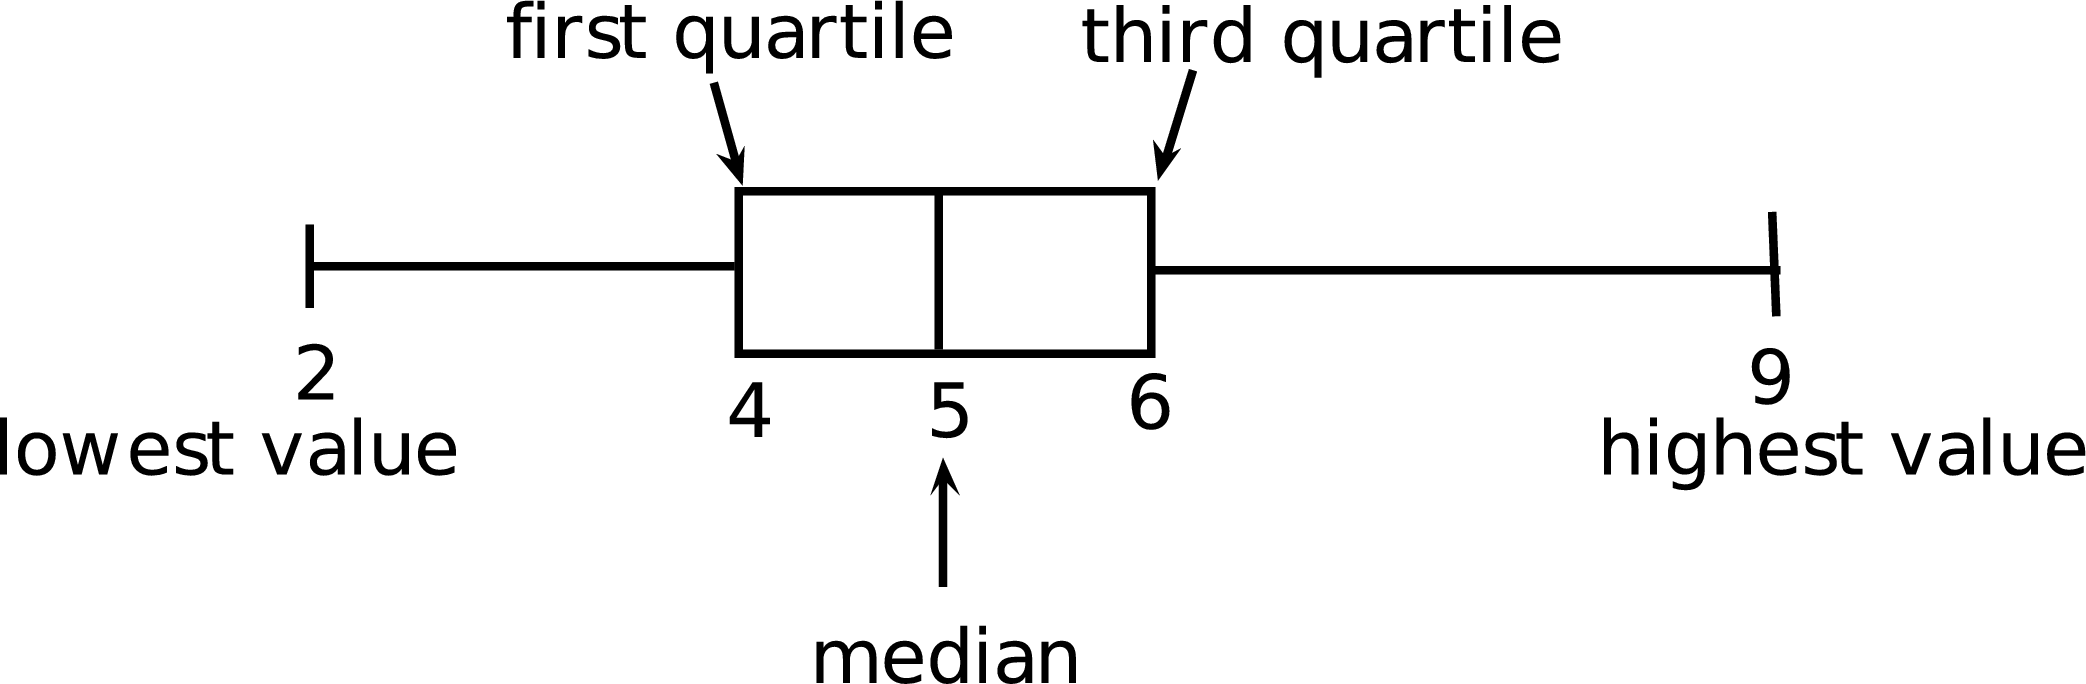
\includegraphics[width=300px]{col11306.imgs/m39400_boxwhisker.png} % m39400;boxwhisker.png;;;6.0;8.5;
      \vspace{2pt}
    \vspace{\rubberspace}\par \begin{cnxcaption}
	  \small \textbf{Figure 16.4: }Main features of a box and whisker plot
	\end{cnxcaption}
    \vspace{.1in}
    \end{center}
 \end{figure}       \par \par
            \label{m39400*eip-742}\vspace{.5cm} 
      \noindent
      \hspace*{-30pt}
\includegraphics[width=0.5in]{col11306.imgs/pspencil2.png}   \raisebox{25mm}{   
      \begin{mdframed}[linewidth=4, leftmargin=40, rightmargin=40]  
      \begin{exercise}
    \noindent\textbf{Exercise 16.9}\label{m39400*eip-570}
  \label{m39400*eip-327}
Draw a box and whisker diagram for the data set:
$x=\{1,25;1,5;2,5;2,5;3,1;3,2;4,1;4,25;4,75;4,8;4,95;5,1\}$.
  \par 
\vspace{5pt}
\label{m39400*eip-402}\noindent\textbf{Solution to Exercise }
  \label{m39400*eip-701}\begin{enumerate}[noitemsep, label=\textbf{Step} \textbf{\arabic*}. ] 
            \leftskip=20pt\rightskip=\leftskip\item \newline
    $\mathrm{Minimum}=1,25$\newline
$\mathrm{Maximum}=5,10$\newline
The position of first quartile is between 3 and 4. \newline
The position of second quartile is between 6 and 7. \newline
The position of third quartile is between 9 and 10. \newline
The data value between 3 and 4 is:
$\frac{1}{2}\left(2,5+2,5\right)=2,5$\newline
The data value between 6 and 7 is:
$\frac{1}{2}\left(3,2+4,1\right)=3,65$\newline
The data value between 9 and 10 is: 
$\frac{1}{2}\left(4,75+4,8\right)=4,775$\item 
    \setcounter{subfigure}{0}
	\begin{figure}[H] % horizontal\label{m39400*uid34553}
    \begin{center}
    \label{m39400*uid34553!!!underscore!!!media}\label{m39400*uid34553!!!underscore!!!printimage}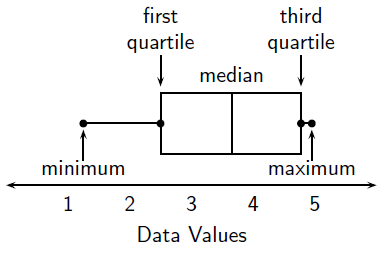
\includegraphics{col11306.imgs/m39400_boxwhisker1.png} % ;boxwhisker1.png;;;6.0;8.5;
      \vspace{2pt}
    \vspace{.1in}
    \end{center}
 \end{figure}       \end{enumerate}
    \end{exercise}
    \end{mdframed}
    }
    \noindent
  \label{m39400*uid86}
            \subsubsection{ Exercises - Summarising Data}
            \nopagebreak
        \label{m39400*id214700}\begin{enumerate}[noitemsep, label=\textbf{\arabic*}. ] 
            \label{m39400*uid87}\item Three sets of data are given:
\label{m39400*id214716}\begin{enumerate}[noitemsep, label=\textbf{\alph*}. ] 
            \label{m39400*uid88}\item \textbf{Data set 1:} 9 12 12 14 16 22 24
\label{m39400*uid89}\item \textbf{Data set 2:} 7 7 8 11 13 15 16 16
\label{m39400*uid90}\item \textbf{Data set 3:} 11 15 16 17 19 19 22 24 27\end{enumerate}
For each one find:
\label{m39400*id214775}\begin{enumerate}[noitemsep, label=\textbf{\alph*}. ] 
            \label{m39400*uid91}\item the range
\label{m39400*uid92}\item the lower quartile
\label{m39400*uid93}\item the interquartile range
\label{m39400*uid94}\item the semi-interquartile range
\label{m39400*uid95}\item the median
\label{m39400*uid96}\item the upper quartile
\end{enumerate}
                \label{m39400*uid97}\item There is 1 sweet in one jar, and 3 in the second jar. The mean number of sweets in the first two jars is 2.
\label{m39400*id214868}\begin{enumerate}[noitemsep, label=\textbf{\alph*}. ] 
            \label{m39400*uid98}\item If the mean number in the first three jars is 3, how many are there in the third jar?
\label{m39400*uid99}\item If the mean number in the first four jars is 4, how many are there in the fourth jar?
\end{enumerate}
                \label{m39400*uid101}\item Find a set of five ages for which the mean age is 5, the modal age is 2 and the median age is 3 years.\newline
\label{m39400*uid102}\item Four friends each have some marbles. They work out that the mean number of marbles they have is 10. One of them leaves. She has 4 marbles. How many marbles do the remaining friends have together?\newline
\item Jason is working in a computer store. He sells the following number of computers each month:
27; 39; 3; 15; 43; 27; 19; 54; 65; 23; 45; 16
Give a five number summary and a box and whisker plot of his sales.\newline
\item Lisa works as a telesales person. She keeps a record of the number of sales she makes each month. The data below show how much she sells each month.
49; 12; 22; 35; 2; 45; 60; 48; 19; 1; 43; 12
Give a five number summary and a box and whisker plot of her sales.\newline
\item Rose has worked in a florists shop for nine months. She sold the following number of wedding bouquets:
16; 14; 8; 12; 6; 5; 3; 5; 7
\label{m39400*id63452}\begin{enumerate}[noitemsep, label=\textbf{\alph*}. ] 
            \item What is the five-number summary of the data?\item Since there is an odd number of data points what do you observe when calculating the five-numbers?\end{enumerate}
\end{enumerate}
\label{m39400*eip-405}We can apply the concepts of mean, median and mode to data that has been grouped. Grouped data does not have individual data points, but rather has the data organized into groups or bins. To calculate the mean we need to add up all the frequencies and divide by the total. We do not know what the actual data values are, so we approximate by choosing the midpoint of each group. We then multiply those midpoint numbers by the frequency. Then we add these numbers together to find the approximate total of the masses. The modal group is the group with the highest frequency. The median group is the group that contains the middle terms.\par \label{m39400*eip-151}Measures of dispersion can also be found for grouped data. The range is found by subtracting the smallest number in the lowest bin from the largest number in the highest bin. The quartiles are found in a similar way to the median.\par \label{m39400*secfhsst!!!underscore!!!id2004}\vspace{.5cm} 
      \noindent
      \hspace*{-30pt}
\includegraphics[width=0.5in]{col11306.imgs/pspencil2.png}   \raisebox{25mm}{   
      \begin{mdframed}[linewidth=4, leftmargin=40, rightmargin=40]  
      \begin{exercise}
    \noindent\textbf{Exercise 16.10:  Mean, Median and Mode for Grouped Data }
        \label{m39400*probfhsst!!!underscore!!!id2005}
        \label{m39400*id214977}Consider the following grouped data and calculate the mean, the modal group and the median group.\par 
    % \textbf{m39400*id214984}\par
          \begin{table}[H]
    % \begin{table}[H]
    % \\ '' '0'
        \begin{center}
      \label{m39400*id214984}
    \noindent
    \tabletail{%
        \hline
        \multicolumn{2}{|p{\mytableboxwidth}|}{\raggedleft \small \sl continued on next page}\\
        \hline
      }
      \tablelasttail{}
      \begin{xtabular}[t]{|l|l|}\hline
        Mass (kg) &
        Frequency% make-rowspan-placeholders
     \tabularnewline\cline{1-1}\cline{2-2}
      %--------------------------------------------------------------------
        41 - 45 &
        7% make-rowspan-placeholders
     \tabularnewline\cline{1-1}\cline{2-2}
      %--------------------------------------------------------------------
        46 - 50 &
        10% make-rowspan-placeholders
     \tabularnewline\cline{1-1}\cline{2-2}
      %--------------------------------------------------------------------
        51 - 55 &
        15% make-rowspan-placeholders
     \tabularnewline\cline{1-1}\cline{2-2}
      %--------------------------------------------------------------------
        56 - 60 &
        12% make-rowspan-placeholders
     \tabularnewline\cline{1-1}\cline{2-2}
      %--------------------------------------------------------------------
        61 - 65 &
        6% make-rowspan-placeholders
     \tabularnewline\cline{1-1}\cline{2-2}
      %--------------------------------------------------------------------
         &
        Total = 50% make-rowspan-placeholders
     \tabularnewline\cline{1-1}\cline{2-2}
      %--------------------------------------------------------------------
    \end{xtabular}
      \end{center}
    \begin{center}{\small\bfseries Table 16.14}\end{center}
    \begin{caption}{\small\bfseries Table 16.14}\end{caption}
\end{table}
    \par
        \vspace{5pt}
        \label{m39400*solfhsst!!!underscore!!!id2044}\noindent\textbf{Solution to Exercise } \label{m39400*listfhsst!!!underscore!!!id2044}\begin{enumerate}[noitemsep, label=\textbf{Step} \textbf{\arabic*}. ] 
            \leftskip=20pt\rightskip=\leftskip\item  
        \label{m39400*id215169}To calculate the mean we need to add up all the masses and divide by 50. We do not know actual masses, so we approximate by choosing the midpoint of each group. We then multiply those midpoint numbers by the frequency. Then we add these numbers together to find the approximate total of the masses. This is show in the table below.\par 
    % \textbf{m39400*id215176}\par
          \begin{table}[H]
    % \begin{table}[H]
    % \\ 'id2999828' '1'
        \begin{center}
      \label{m39400*id215176}
    \noindent
    \tabletail{%
        \hline
        \multicolumn{4}{|p{\mytableboxwidth}|}{\raggedleft \small \sl continued on next page}\\
        \hline
      }
      \tablelasttail{}
      \begin{xtabular}[t]{|l|l|l|l|}\hline
        Mass (kg) &
        Midpoint &
        Frequency &
        Midpt $\ensuremath{\times}$ Freq% make-rowspan-placeholders
     \tabularnewline\cline{1-1}\cline{2-2}\cline{3-3}\cline{4-4}
      %--------------------------------------------------------------------
        41 - 45 &
        (41+45)/2 = 43 &
        7 &
        43 $\ensuremath{\times}$ 7 = 301% make-rowspan-placeholders
     \tabularnewline\cline{1-1}\cline{2-2}\cline{3-3}\cline{4-4}
      %--------------------------------------------------------------------
        46 - 50 &
        48 &
        10 &
        480% make-rowspan-placeholders
     \tabularnewline\cline{1-1}\cline{2-2}\cline{3-3}\cline{4-4}
      %--------------------------------------------------------------------
        51 - 55 &
        53 &
        15 &
        795% make-rowspan-placeholders
     \tabularnewline\cline{1-1}\cline{2-2}\cline{3-3}\cline{4-4}
      %--------------------------------------------------------------------
        56 - 60 &
        58 &
        12 &
        696% make-rowspan-placeholders
     \tabularnewline\cline{1-1}\cline{2-2}\cline{3-3}\cline{4-4}
      %--------------------------------------------------------------------
        61 - 65 &
        63 &
        6 &
        378% make-rowspan-placeholders
     \tabularnewline\cline{1-1}\cline{2-2}\cline{3-3}\cline{4-4}
      %--------------------------------------------------------------------
         &
         &
        Total = 50 &
        Total = 2650% make-rowspan-placeholders
     \tabularnewline\cline{1-1}\cline{2-2}\cline{3-3}\cline{4-4}
      %--------------------------------------------------------------------
    \end{xtabular}
      \end{center}
    \begin{center}{\small\bfseries Table 16.15}\end{center}
    \begin{caption}{\small\bfseries Table 16.15}\end{caption}
\end{table}
    \par
        \item  
        \label{m39400*id215455}The mean = $\frac{2650}{50}=53$.\par 
        \label{m39400*id215478}The modal group is the group 51 - 53 because it has the highest frequency.\par 
        \label{m39400*id215484}The median group is the group 51 - 53, since the 25th and 26th terms are contained within this group.\par 
\end{enumerate}
    \end{exercise}
    \end{mdframed}
    }
    \noindent
\label{m39400*secfhsst!!!underscore!!!id2103}
\par \raisebox{-0.2em}{
\includegraphics[height=1em]{../icons/www.pdf}} Find the answers with the shortcodes:
 \par \begin{tabular}[h]{cccccc}
 (1.) l48  &  (2.) l49  &  (3.) l4X  &  (4.) l4I  &  (5.) l2Q  &  (6.) l2U  &  (7.) l2P  & \end{tabular}
            \subsubsection{  More mean, modal and median group exercises. }
            \nopagebreak
        \label{m39400*id215497}In each data set given, find the mean, the modal group and the median group.\par 
        \label{m39400*id215504}\begin{enumerate}[noitemsep, label=\textbf{\arabic*}. ] 
            \label{m39400*uid103}\item Times recorded when learners played a game.
    % \textbf{m39400*id215519}\par
          \begin{table}[H]
    % \begin{table}[H]
    % \\ 'id3000062' '1'
        \begin{center}
      \label{m39400*id215519}
    \noindent
    \tabletail{%
        \hline
        \multicolumn{2}{|p{\mytableboxwidth}|}{\raggedleft \small \sl continued on next page}\\
        \hline
      }
      \tablelasttail{}
      \begin{xtabular}[t]{|l|l|}\hline
        Time in seconds &
        Frequency% make-rowspan-placeholders
     \tabularnewline\cline{1-1}\cline{2-2}
      %--------------------------------------------------------------------
        36 - 45 &
        5% make-rowspan-placeholders
     \tabularnewline\cline{1-1}\cline{2-2}
      %--------------------------------------------------------------------
        46 - 55 &
        11% make-rowspan-placeholders
     \tabularnewline\cline{1-1}\cline{2-2}
      %--------------------------------------------------------------------
        56 - 65 &
        15% make-rowspan-placeholders
     \tabularnewline\cline{1-1}\cline{2-2}
      %--------------------------------------------------------------------
        66 - 75 &
        26% make-rowspan-placeholders
     \tabularnewline\cline{1-1}\cline{2-2}
      %--------------------------------------------------------------------
        76 - 85 &
        19% make-rowspan-placeholders
     \tabularnewline\cline{1-1}\cline{2-2}
      %--------------------------------------------------------------------
        86 - 95 &
        13% make-rowspan-placeholders
     \tabularnewline\cline{1-1}\cline{2-2}
      %--------------------------------------------------------------------
        96 - 105 &
        6% make-rowspan-placeholders
     \tabularnewline\cline{1-1}\cline{2-2}
      %--------------------------------------------------------------------
    \end{xtabular}
      \end{center}
    \begin{center}{\small\bfseries Table 16.16}\end{center}
    \begin{caption}{\small\bfseries Table 16.16}\end{caption}
\end{table}
    \par
          \label{m39400*uid104}\item The following data were collected from a group of learners.
    % \textbf{m39400*id215730}\par
          \begin{table}[H]
    % \begin{table}[H]
    % \\ 'id3000142' '1'
        \begin{center}
      \label{m39400*id215730}
    \noindent
    \tabletail{%
        \hline
        \multicolumn{2}{|p{\mytableboxwidth}|}{\raggedleft \small \sl continued on next page}\\
        \hline
      }
      \tablelasttail{}
      \begin{xtabular}[t]{|l|l|}\hline
        Mass in kilograms &
        Frequency% make-rowspan-placeholders
     \tabularnewline\cline{1-1}\cline{2-2}
      %--------------------------------------------------------------------
        41 - 45 &
        3% make-rowspan-placeholders
     \tabularnewline\cline{1-1}\cline{2-2}
      %--------------------------------------------------------------------
        46 - 50 &
        5% make-rowspan-placeholders
     \tabularnewline\cline{1-1}\cline{2-2}
      %--------------------------------------------------------------------
        51 - 55 &
        8% make-rowspan-placeholders
     \tabularnewline\cline{1-1}\cline{2-2}
      %--------------------------------------------------------------------
        56 - 60 &
        12% make-rowspan-placeholders
     \tabularnewline\cline{1-1}\cline{2-2}
      %--------------------------------------------------------------------
        61 - 65 &
        14% make-rowspan-placeholders
     \tabularnewline\cline{1-1}\cline{2-2}
      %--------------------------------------------------------------------
        66 - 70 &
        9% make-rowspan-placeholders
     \tabularnewline\cline{1-1}\cline{2-2}
      %--------------------------------------------------------------------
        71 - 75 &
        7% make-rowspan-placeholders
     \tabularnewline\cline{1-1}\cline{2-2}
      %--------------------------------------------------------------------
        76 - 80 &
        2% make-rowspan-placeholders
     \tabularnewline\cline{1-1}\cline{2-2}
      %--------------------------------------------------------------------
    \end{xtabular}
      \end{center}
    \begin{center}{\small\bfseries Table 16.17}\end{center}
    \begin{caption}{\small\bfseries Table 16.17}\end{caption}
\end{table}
    \par
          \end{enumerate}
  \label{m39400**end}
\par \raisebox{-0.2em}{
\includegraphics[height=1em]{../icons/www.pdf}} Find the answers with the shortcodes:
 \par \begin{tabular}[h]{cccccc}
 (1.) l45  &  (2.) l4N  & \end{tabular}
%          \section{ Bias, error and misuse}
%     \nopagebreak
%             \label{m39404} $ \hspace{-5pt}\begin{array}{cccccccccccc}   \end{array} $ \hspace{2 pt}\raisebox{-0.2em}{
\includegraphics[height=1em]{../icons/www.pdf}} {(section shortcode: MG10117 )} \par 
%     
%     
%     
%     \label{m39404*eip-820}
%             \subsection{ Bias and error in measurements}
%             \nopagebreak
%             \label{m39404*eip-910}
% All measurements have some error associated with them. Random errors occur in all data sets and are sometimes known as non-systematic errors. Random errors can arise from estimation of data values, imprecision of instruments, etc. For example if you are reading lengths off a ruler, random errors will arise in each measurement as a result of estimating between which two lines the length lies. Bias is also sometimes known as systematic error. Bias in a data set is where a value is consistently under or overestimated. Bias can arise from forgetting to take into account a correction factor or from instruments that are not properly calibrated (calibration is the process of marking off predefined measurements). Bias leads to a sample mean that is either lower or higher than the true mean. 
\par 
    \label{m39404*eip-443}
            \section{ Applications}
            \nopagebreak
            \label{m39404*eip-493}Many people take statistics and just blindly apply it to life or quote it. This, however, is not wise since the data that led to the statistics also needs to be considered. A well known example of several sets of data that lead to the same statistical analysis (the process of examining data and determining values such as central tendency, etc.) but are in fact very different is Anscombe's quartet. This is shown in . In Grade 11 you will learn about the methods used to represent data graphically. For now, however, you should simply appreciate the fact that we can plot data values on the Cartesian plane in a similar way to plotting graphs. If each of the datasets in Anscombe's quartet are analysed statistically, then one finds that the mean, variance, correlation and linear regression (these terms will be explained in later grades) are identical. If, instead of analysing the data statistically, we simply plot the data points we can see that the data sets are very different. This example shows us that it is very important to consider the underlying data set as well as the statistics that we obtain from the data. We cannot simply assume that just because we know the statistics of a data set, we know what the data set is telling us. For general interest, some of the ways that statistics and data can be misinterpreted are given in the following extension section.   
    \setcounter{subfigure}{0}
	\begin{figure}[H] % horizontal\label{m39404*uid3453}
    \begin{center}
    \label{m39404*uid3453!!!underscore!!!media}\label{m39404*uid3453!!!underscore!!!printimage}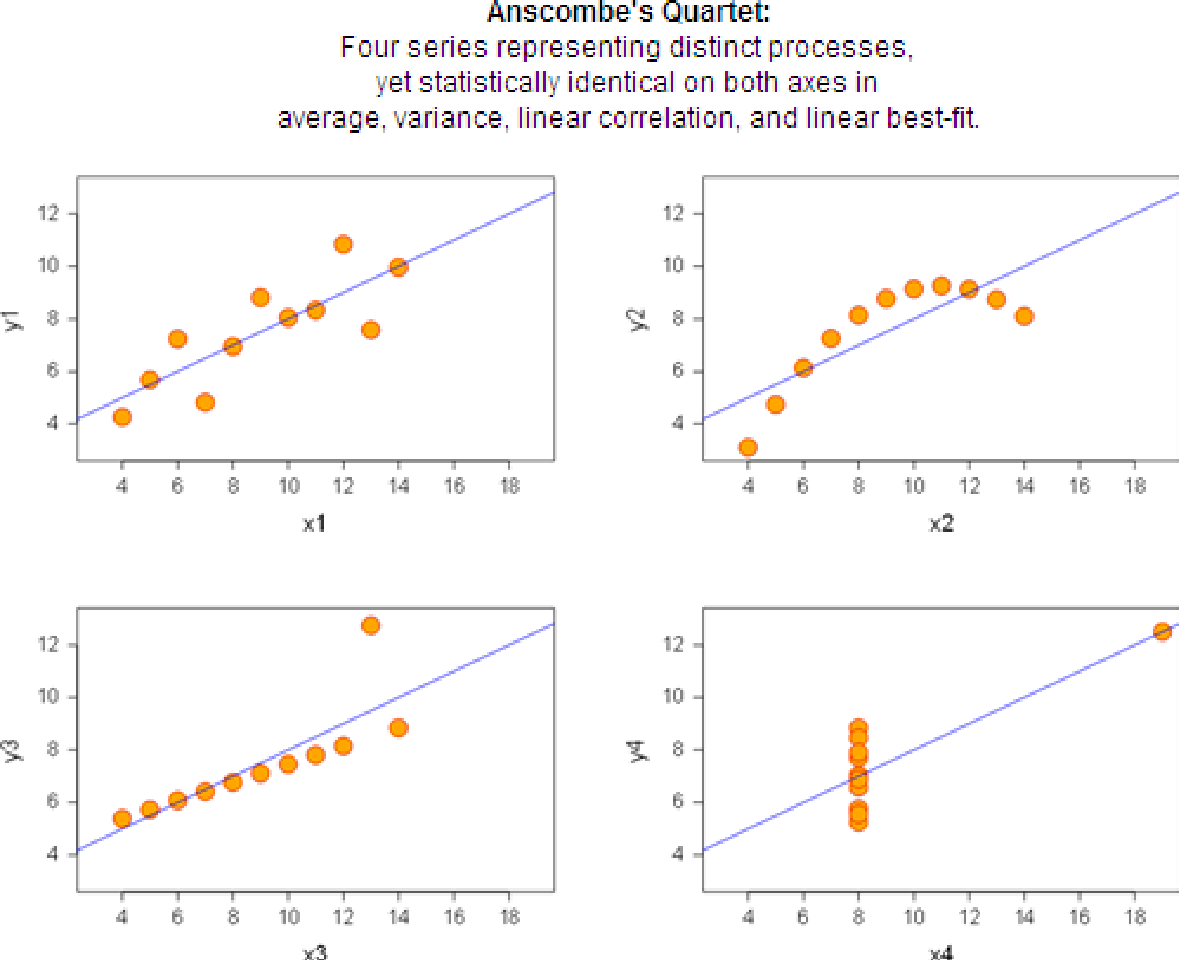
\includegraphics[width=300px]{col11306.imgs/m39404_anscombe.png} % m39404;anscombe.png;;;6.0;8.5;
      \vspace{2pt}
    \vspace{\rubberspace}\par \begin{cnxcaption}
	  \small \textbf{Figure 16.6: }Anscombe's quartet
	\end{cnxcaption}
    \vspace{.1in}
    \end{center}
 \end{figure}       \par 
\label{m39404*cid8}
%             \subsection{ Misuse of Statistics - For enrichment, not in CAPS}
            \nopagebreak
      \label{m39404*id215969}In many cases groups can gain an advantage by misleading people with the misuse of statistics. Companies misuse statistics to attempt to show that they are performing better than a competitor, advertisers abuse statistics to try to convince you to buy their product, researchers misuse statistics to attempt to show that their data is of better quality than it really is, etc.\par 
      \label{m39404*id215973}Common techniques used include:\par 
      \label{m39404*id215979}\begin{itemize}[noitemsep]
            \label{m39404*uid105}\item Three dimensional graphs.
\label{m39404*uid106}\item Axes that do not start at zero.
\label{m39404*uid107}\item Axes without scales.
\label{m39404*uid108}\item Graphic images that convey a negative or positive mood.
\label{m39404*uid109}\item Assumption that a correlation shows a necessary causality.
\label{m39404*uid110}\item Using statistics that are not truly representative of the entire population.
\label{m39404*uid111}\item Using misconceptions of mathematical concepts
\end{itemize}
      \label{m39404*id216070}For example, the following pairs of graphs show identical information but look very different. Explain why.\par 
      \label{m39404*id216074}
    \setcounter{subfigure}{0}
	\begin{figure}[H] % horizontal\label{m39404*id216077}
    \begin{center}
    \label{m39404*id216077!!!underscore!!!media}\label{m39404*id216077!!!underscore!!!printimage}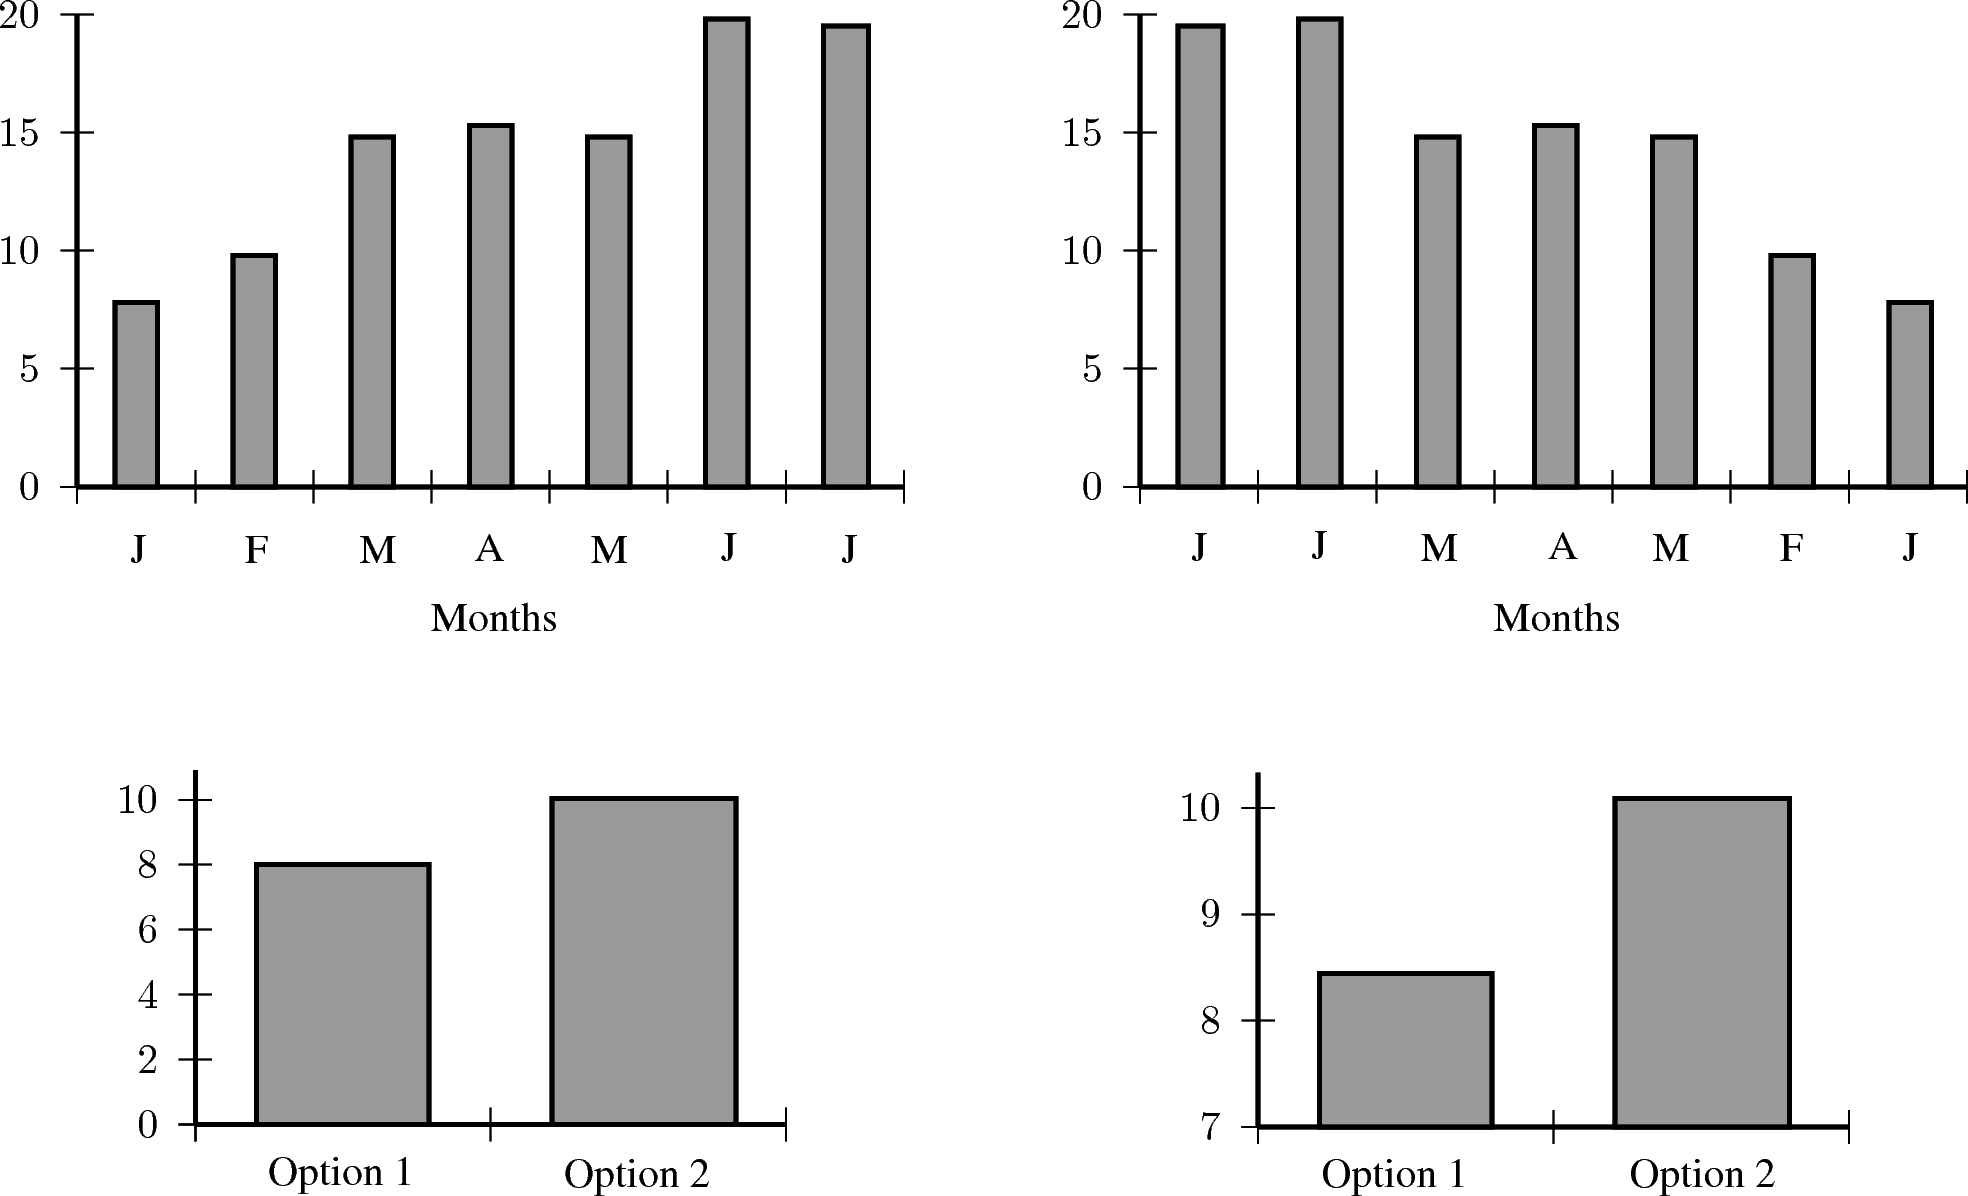
\includegraphics{col11306.imgs/m39404_MG10C16_010.png} % m39404;MG10C16\_010.png;;;6.0;8.5;
      \vspace{2pt}
    \vspace{.1in}
    \end{center}
 \end{figure}       
      \par 
      \label{m39404*uid112}
            \subsubsection{ Exercises - Application of Statistics}
            \nopagebreak
        \label{m39404*id216093}\begin{enumerate}[noitemsep, label=\textbf{\arabic*}. ] 
            \label{m39404*uid113}\item A company has tried to give a visual representation of the increase in their earnings from one year to the next. Does the graph below convince you? Critically analyse the graph.
    \setcounter{subfigure}{0}
	\begin{figure}[H] % horizontal\label{m39404*id216113}
    \begin{center}
    \label{m39404*id216113!!!underscore!!!media}\label{m39404*id216113!!!underscore!!!printimage}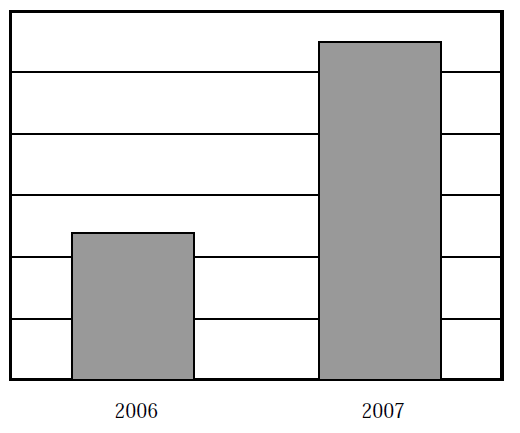
\includegraphics[width=300px]{col11306.imgs/m39404_MG10C16_011.png} % m39404;MG10C16\_011.png;;;6.0;8.5;
      \vspace{2pt}
    \vspace{.1in}
    \end{center}
 \end{figure}               \label{m39404*uid114}\item In a study conducted on a busy highway, data was collected about drivers breaking the speed limit and the colour of the car they were driving. The data were collected during a 20 minute time interval during the middle of the day, and are presented in a table and pie chart below.
\label{m39404*id216251}\begin{itemize}[noitemsep]
            \label{m39404*uid115}\item Conclusions made by a novice based on the data are summarised as follows:
\label{m39404*uid116}\item ``People driving white cars are more likely to break the speed limit.''
\label{m39404*uid117}\item ``Drivers in blue and red cars are more likely to stick to the speed limit.''
\label{m39404*uid118}\item Do you agree with these conclusions? Explain.
\end{itemize}
                \label{m39404*uid119}\item A record label produces a graphic, showing their advantage in sales over their competitors. Identify at least three devices they have used to influence and mislead the readers impression.
    \setcounter{subfigure}{0}
	\begin{figure}[H] % horizontal\label{m39404*id216327}
    \begin{center}
    \label{m39404*id216327!!!underscore!!!media}\label{m39404*id216327!!!underscore!!!printimage}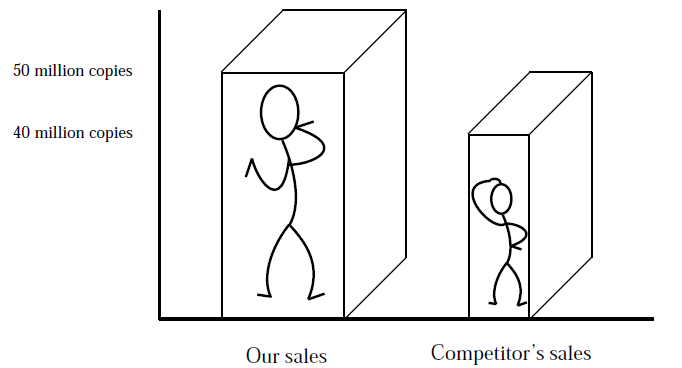
\includegraphics[width=300px]{col11306.imgs/m39404_MG10C16_013.png} % m39404;MG10C16\_013.png;;;6.0;8.5;
      \vspace{2pt}
    \vspace{.1in}
    \end{center}
 \end{figure}               \label{m39404*uid120}\item In an effort to discredit their competition, a tour bus company prints the graph shown below. Their claim is that the competitor is losing business. Can you think of a better explanation?
    \setcounter{subfigure}{0}
	\begin{figure}[H] % horizontal\label{m39404*id216351}
    \begin{center}
    \label{m39404*id216351!!!underscore!!!media}\label{m39404*id216351!!!underscore!!!printimage}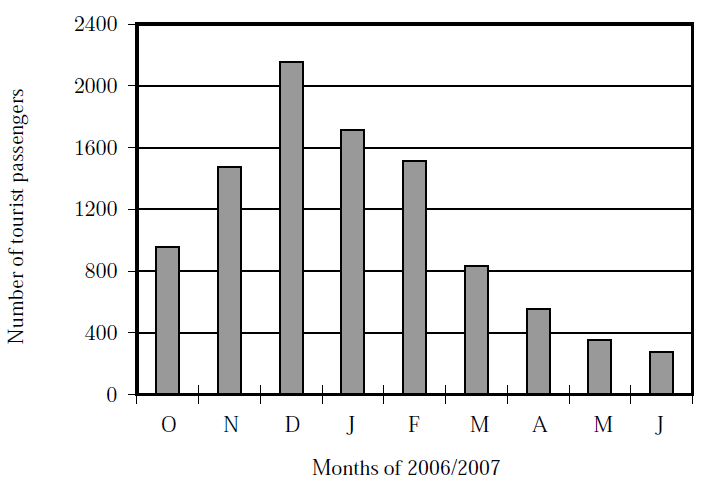
\includegraphics[width=300px]{col11306.imgs/m39404_MG10C16_014.png} % m39404;MG10C16\_014.png;;;6.0;8.5;
      \vspace{2pt}
    \vspace{.1in}
    \end{center}
 \end{figure}               \label{m39404*uid121}\item To test a theory, 8 different offices were monitored for noise levels and productivity of the employees in the office. The results are graphed below.
    \setcounter{subfigure}{0}
	\begin{figure}[H] % horizontal\label{m39404*id216374}
    \begin{center}
    \label{m39404*id216374!!!underscore!!!media}\label{m39404*id216374!!!underscore!!!printimage}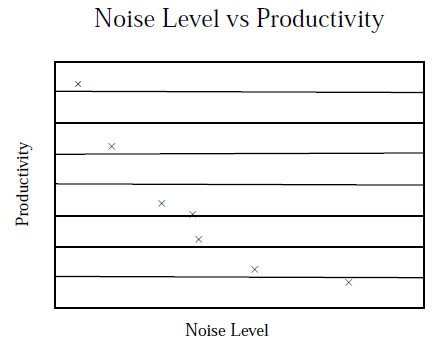
\includegraphics[width=300px]{col11306.imgs/m39404_MG10C16_015.png} % m39404;MG10C16\_015.png;;;6.0;8.5;
      \vspace{2pt}
    \vspace{.1in}
    \end{center}
 \end{figure}       
The following statement was then made:
``If an office environment is noisy, this leads to poor productivity.''
Explain the flaws in this thinking.\newline
\end{enumerate}
\label{m39404*cid9}
\par \raisebox{-0.2em}{
\includegraphics[height=1em]{../icons/www.pdf}} Find the answers with the shortcodes:
 \par \begin{tabular}[h]{cccccc}
 (1.) l4R  &  (2.) l4n  &  (3.) l4Q  &  (4.) l4U  &  (5.) l4P  & \end{tabular}
            \subsection{ End of chapter summary}
            \nopagebreak
            \label{m39404*id216407}\begin{itemize}[noitemsep, label=\textbullet{}]
            \item Data types can be divided into primary and secondary data. Primary data may be further divided into qualitative and quantitative data.\label{m39404*id97322}\item We use the following as measures of central tendency:\label{m39404*id67453}\begin{itemize}[noitemsep]
            \label{m39404*uid122}\item The mean of a data set, $x$, denoted by $\overline{x}$, is the average of the data values, and is calculated as:
\label{m39404*id216451}\nopagebreak\noindent{}
    \begin{equation}
    \overline{x}=\frac{\mathrm{sum\; of\; values}}{\mathrm{number\; of\; values}}\tag{16.7}
      \end{equation}
    \label{m39404*uid123}\item The median is the centre data value in a data set that has been ordered from lowest to highest
\label{m39404*uid12454}\item The mode is the data value that occurs most often in a data set.
\end{itemize}
        \label{m39404*id973243222}\item The following are measures of dispersion:\label{m39404*id6743453453}\begin{itemize}[noitemsep]
            \label{m39404*uid12542}\item The range of a data set is the difference between the lowest value and the highest value in the set. \label{m39404*uid123543}\item Quartiles are the three data values that divide an ordered data set into four groups containing equal numbers of data values. The median is the second quartile. 
\label{m39404*uid124}\item Percentiles are the 99 data values that divide a data set into 100 groups. 
\label{m39404*uid124342}\item The inter quartile range is a measure which provides information about the spread of a data set, and is calculated by subtracting the first quartile from the third quartile, giving the range of the middle half of the data set, trimming off the lowest and highest quarters, i.e. ${Q}_{3}-{Q}_{1}$. Half of this value is the semi-interquartile range.\end{itemize}
        \item The five number summary is a way to summarise data. A box and whisker plot is a graphical representation of the five number summary.\item Random errors are found in all sets of data and arise from estimating data values. Bias or systematic error occurs when you consistently under or over estimate data values.\item You must always consider the data and the statistics that summarise the data\end{itemize}
    \label{m39404*cid10}
            \subsection{ End of Chapter Exercises}
            \nopagebreak
      \label{m39404*id216570}\begin{enumerate}[noitemsep, label=\textbf{\arabic*}. ] 
            \label{m39404*uid125}\item Calculate the mean, median, and mode of Data Set 3.\newline
\label{m39404*uid126}\item The tallest 7 trees in a park have heights in metres of 41, 60, 47, 42, 44, 42, and 47. Find the median of their heights.\newline
\label{m39404*uid127}\item The students in Bjorn's class have the following ages: 5, 6, 7, 5, 4, 6, 6, 6, 7, 4. Find the mode of their ages.\newline
\label{m39404*uid132}\item An engineering company has designed two different types of engines for motorbikes. The two different motorbikes are tested for the time it takes (in seconds) for them to accelerate from 0 km/h to 60 km/h.
    % \textbf{m39404*id217268}\par
          \begin{table}[H]
    % \begin{table}[H]
    % \\ 'id3001214' '1'
        \begin{center}
      \label{m39404*id217268}
    \noindent
    \tabletail{%
        \hline
        \multicolumn{12}{|p{\mytableboxwidth}|}{\raggedleft \small \sl continued on next page}\\
        \hline
      }
      \tablelasttail{}
      \begin{xtabular}[t]{|l|l|l|l|l|l|l|l|l|l|l|l|}\hline
         &
        Test 1 &
        Test 2 &
        Test 3 &
        Test 4 &
        Test 5 &
        Test 6 &
        Test 7 &
        Test 8 &
        Test 9 &
        Test 10 &
        Average% make-rowspan-placeholders
     \tabularnewline\cline{1-1}\cline{2-2}\cline{3-3}\cline{4-4}\cline{5-5}\cline{6-6}\cline{7-7}\cline{8-8}\cline{9-9}\cline{10-10}\cline{11-11}\cline{12-12}
      %--------------------------------------------------------------------
        Bike 1 &
        1.55 &
        1.00 &
        0.92 &
        0.80 &
        1.49 &
        0.71 &
        1.06 &
        0.68 &
        0.87 &
        1.09 &
        % make-rowspan-placeholders
     \tabularnewline\cline{1-1}\cline{2-2}\cline{3-3}\cline{4-4}\cline{5-5}\cline{6-6}\cline{7-7}\cline{8-8}\cline{9-9}\cline{10-10}\cline{11-11}\cline{12-12}
      %--------------------------------------------------------------------
        Bike 2 &
        0.9 &
        1.0 &
        1.1 &
        1.0 &
        1.0 &
        0.9 &
        0.9 &
        1.0 &
        0.9 &
        1.1 &
        % make-rowspan-placeholders
     \tabularnewline\cline{1-1}\cline{2-2}\cline{3-3}\cline{4-4}\cline{5-5}\cline{6-6}\cline{7-7}\cline{8-8}\cline{9-9}\cline{10-10}\cline{11-11}\cline{12-12}
      %--------------------------------------------------------------------
    \end{xtabular}
      \end{center}
    \begin{center}{\small\bfseries Table 16.18}\end{center}
    \begin{caption}{\small\bfseries Table 16.18}\end{caption}
\end{table}
    \par
  \label{m39404*id217423}\begin{enumerate}[noitemsep, label=\textbf{\alph*}. ] 
            \label{m39404*uid133}\item What measure of central tendency should be used for this information?
\label{m39404*uid134}\item Calculate the average you chose in the previous question for each motorbike.
\label{m39404*uid135}\item Which motorbike would you choose based on this information? Take note of accuracy of the numbers from each set of tests.
\end{enumerate}
                \label{m39404*uid136}\item The heights of 40 learners are given below.
    % \textbf{m39404*id217478}\par
          \begin{table}[H]
    % \begin{table}[H]
    % \\ 'id3001360' '1'
        \begin{center}
      \label{m39404*id217478}
    \noindent
    \tabletail{%
        \hline
        \multicolumn{10}{|p{\mytableboxwidth}|}{\raggedleft \small \sl continued on next page}\\
        \hline
      }
      \tablelasttail{}
      \begin{xtabular}[t]{|l|l|l|l|l|l|l|l|l|l|}\hline
        154 &
        140 &
        145 &
        159 &
        150 &
        132 &
        149 &
        150 &
        138 &
        152% make-rowspan-placeholders
     \tabularnewline\cline{1-1}\cline{2-2}\cline{3-3}\cline{4-4}\cline{5-5}\cline{6-6}\cline{7-7}\cline{8-8}\cline{9-9}\cline{10-10}
      %--------------------------------------------------------------------
        141 &
        132 &
        169 &
        173 &
        139 &
        161 &
        163 &
        156 &
        157 &
        171% make-rowspan-placeholders
     \tabularnewline\cline{1-1}\cline{2-2}\cline{3-3}\cline{4-4}\cline{5-5}\cline{6-6}\cline{7-7}\cline{8-8}\cline{9-9}\cline{10-10}
      %--------------------------------------------------------------------
        168 &
        166 &
        151 &
        152 &
        132 &
        142 &
        170 &
        162 &
        146 &
        152% make-rowspan-placeholders
     \tabularnewline\cline{1-1}\cline{2-2}\cline{3-3}\cline{4-4}\cline{5-5}\cline{6-6}\cline{7-7}\cline{8-8}\cline{9-9}\cline{10-10}
      %--------------------------------------------------------------------
        142 &
        150 &
        161 &
        138 &
        170 &
        131 &
        145 &
        146 &
        147 &
        160% make-rowspan-placeholders
     \tabularnewline\cline{1-1}\cline{2-2}\cline{3-3}\cline{4-4}\cline{5-5}\cline{6-6}\cline{7-7}\cline{8-8}\cline{9-9}\cline{10-10}
      %--------------------------------------------------------------------
    \end{xtabular}
      \end{center}
    \begin{center}{\small\bfseries Table 16.19}\end{center}
    \begin{caption}{\small\bfseries Table 16.19}\end{caption}
\end{table}
    \par
  \label{m39404*id217711}\begin{enumerate}[noitemsep, label=\textbf{\alph*}. ] 
            \label{m39404*uid137}\item Set up a frequency table using 6 intervals.
\label{m39404*uid138}\item Calculate the approximate mean.
\label{m39404*uid139}\item Determine the mode.
\label{m39404*uid140}\item How many learners are taller than your approximate average in (b)?
\end{enumerate}
                \label{m39404*uid141}\item In a traffic survey, a random sample of 50 motorists were asked the distance they drove to work daily. This information is shown in the table below.
    % \textbf{m39404*id217778}\par
          \begin{table}[H]
    % \begin{table}[H]
    % \\ 'id3001514' '1'
        \begin{center}
      \label{m39404*id217778}
    \noindent
    \tabletail{%
        \hline
        \multicolumn{10}{|p{\mytableboxwidth}|}{\raggedleft \small \sl continued on next page}\\
        \hline
      }
      \tablelasttail{}
      \begin{xtabular}[t]{|l|l|l|l|l|l|l|l|l|l|}\hline
        Distance in km &
        1-5 &
        6-10 &
        11-15 &
        16-20 &
        21-25 &
        26-30 &
        31-35 &
        36-40 &
        41-45% make-rowspan-placeholders
     \tabularnewline\cline{1-1}\cline{2-2}\cline{3-3}\cline{4-4}\cline{5-5}\cline{6-6}\cline{7-7}\cline{8-8}\cline{9-9}\cline{10-10}
      %--------------------------------------------------------------------
        Frequency &
        4 &
        5 &
        9 &
        10 &
        7 &
        8 &
        3 &
        2 &
        2% make-rowspan-placeholders
     \tabularnewline\cline{1-1}\cline{2-2}\cline{3-3}\cline{4-4}\cline{5-5}\cline{6-6}\cline{7-7}\cline{8-8}\cline{9-9}\cline{10-10}
      %--------------------------------------------------------------------
    \end{xtabular}
      \end{center}
    \begin{center}{\small\bfseries Table 16.20}\end{center}
    \begin{caption}{\small\bfseries Table 16.20}\end{caption}
\end{table}
    \par
  \label{m39404*id217956}\begin{enumerate}[noitemsep, label=\textbf{\alph*}. ] 
            \label{m39404*uid142}\item Find the approximate mean.
\label{m39404*uid143}\item What percentage of samples drove
\label{m39404*id217984}\begin{enumerate}[noitemsep, label=\textbf{\roman*}. ] 
            \label{m39404*uid144}\item less than 16 km?
\label{m39404*uid145}\item more than 30 km?
\label{m39404*uid146}\item between 16 km and 30 km daily?
\end{enumerate}
        \end{enumerate}
                \label{m39404*uid147}\item A company wanted to evaluate the training programme in its factory. They gave the same task to trained and untrained employees and timed each one in seconds.
    % \textbf{m39404*id218040}\par
          \begin{table}[H]
    % \begin{table}[H]
    % \\ 'id3001644' '1'
        \begin{center}
      \label{m39404*id218040}
    \noindent
    \tabletail{%
        \hline
        \multicolumn{6}{|p{\mytableboxwidth}|}{\raggedleft \small \sl continued on next page}\\
        \hline
      }
      \tablelasttail{}
      \begin{xtabular}[t]{|l|l|l|l|l|l|}\hline
        \textbf{Trained} &
        121 &
        137 &
        131 &
        135 &
        130% make-rowspan-placeholders
     \tabularnewline\cline{1-1}\cline{2-2}\cline{3-3}\cline{4-4}\cline{5-5}\cline{6-6}
      %--------------------------------------------------------------------
         &
        128 &
        130 &
        126 &
        132 &
        127% make-rowspan-placeholders
     \tabularnewline\cline{1-1}\cline{2-2}\cline{3-3}\cline{4-4}\cline{5-5}\cline{6-6}
      %--------------------------------------------------------------------
         &
        129 &
        120 &
        118 &
        125 &
        134% make-rowspan-placeholders
     \tabularnewline\cline{1-1}\cline{2-2}\cline{3-3}\cline{4-4}\cline{5-5}\cline{6-6}
      %--------------------------------------------------------------------
        \textbf{Untrained} &
        135 &
        142 &
        126 &
        148 &
        145% make-rowspan-placeholders
     \tabularnewline\cline{1-1}\cline{2-2}\cline{3-3}\cline{4-4}\cline{5-5}\cline{6-6}
      %--------------------------------------------------------------------
         &
        156 &
        152 &
        153 &
        149 &
        145% make-rowspan-placeholders
     \tabularnewline\cline{1-1}\cline{2-2}\cline{3-3}\cline{4-4}\cline{5-5}\cline{6-6}
      %--------------------------------------------------------------------
         &
        144 &
        134 &
        139 &
        140 &
        142% make-rowspan-placeholders
     \tabularnewline\cline{1-1}\cline{2-2}\cline{3-3}\cline{4-4}\cline{5-5}\cline{6-6}
      %--------------------------------------------------------------------
    \end{xtabular}
      \end{center}
    \begin{center}{\small\bfseries Table 16.21}\end{center}
    \begin{caption}{\small\bfseries Table 16.21}\end{caption}
\end{table}
    \par
  \label{m39404*id218292}\begin{enumerate}[noitemsep, label=\textbf{\alph*}. ] 
            \label{m39404*uid148}\item Find the medians and quartiles for both sets of data.
\label{m39404*uid149}\item Find the Interquartile Range for both sets of data.
\label{m39404*uid150}\item Comment on the results.
\end{enumerate}
                \label{m39404*uid151}\item A small firm employs nine people. The annual salaries of the employers are:
    % \textbf{m39404*id218346}\par
          \begin{table}[H]
    % \begin{table}[H]
    % \\ 'id3001791' '1'
        \begin{center}
      \label{m39404*id218346}
    \noindent
    \tabletail{%
        \hline
        \multicolumn{3}{|p{\mytableboxwidth}|}{\raggedleft \small \sl continued on next page}\\
        \hline
      }
      \tablelasttail{}
      \begin{xtabular}[t]{|l|l|l|}\hline
        R600 000 &
        R250 000 &
        R200 000% make-rowspan-placeholders
     \tabularnewline\cline{1-1}\cline{2-2}\cline{3-3}
      %--------------------------------------------------------------------
        R120 000 &
        R100 000 &
        R100 000% make-rowspan-placeholders
     \tabularnewline\cline{1-1}\cline{2-2}\cline{3-3}
      %--------------------------------------------------------------------
        R100 000 &
        R90 000 &
        R80 000% make-rowspan-placeholders
     \tabularnewline\cline{1-1}\cline{2-2}\cline{3-3}
      %--------------------------------------------------------------------
    \end{xtabular}
      \end{center}
    \begin{center}{\small\bfseries Table 16.22}\end{center}
    \begin{caption}{\small\bfseries Table 16.22}\end{caption}
\end{table}
    \par
  \label{m39404*id218444}\begin{enumerate}[noitemsep, label=\textbf{\alph*}. ] 
            \label{m39404*uid152}\item Find the mean of these salaries.
\label{m39404*uid153}\item Find the mode.
\label{m39404*uid154}\item Find the median.
\label{m39404*uid155}\item Of these three figures, which would you use for negotiating salary increases if you were a trade union official? Why?
\end{enumerate}
                \label{m39404*uid156}\item The marks for a particular class test are listed here:
    % \textbf{m39404*id218511}\par
          \begin{table}[H]
    % \begin{table}[H]
    % \\ 'id3001881' '1'
        \begin{center}
      \label{m39404*id218511}
    \noindent
    \tabletail{%
        \hline
        \multicolumn{10}{|p{\mytableboxwidth}|}{\raggedleft \small \sl continued on next page}\\
        \hline
      }
      \tablelasttail{}
      \begin{xtabular}[t]{|l|l|l|l|l|l|l|l|l|l|}\hline
        67 &
        58 &
        91 &
        67 &
        58 &
        82 &
        71 &
        51 &
        60 &
        84% make-rowspan-placeholders
     \tabularnewline\cline{1-1}\cline{2-2}\cline{3-3}\cline{4-4}\cline{5-5}\cline{6-6}\cline{7-7}\cline{8-8}\cline{9-9}\cline{10-10}
      %--------------------------------------------------------------------
        31 &
        67 &
        96 &
        64 &
        78 &
        71 &
        87 &
        78 &
        89 &
        38% make-rowspan-placeholders
     \tabularnewline\cline{1-1}\cline{2-2}\cline{3-3}\cline{4-4}\cline{5-5}\cline{6-6}\cline{7-7}\cline{8-8}\cline{9-9}\cline{10-10}
      %--------------------------------------------------------------------
        69 &
        62 &
        60 &
        73 &
        60 &
        87 &
        71 &
        49 &
         &
        % make-rowspan-placeholders
     \tabularnewline\cline{1-1}\cline{2-2}\cline{3-3}\cline{4-4}\cline{5-5}\cline{6-6}\cline{7-7}\cline{8-8}\cline{9-9}\cline{10-10}
      %--------------------------------------------------------------------
    \end{xtabular}
      \end{center}
    \begin{center}{\small\bfseries Table 16.23}\end{center}
    \begin{caption}{\small\bfseries Table 16.23}\end{caption}
\end{table}
    \par
  \label{m39404*eip-id1167180050127}Complete the frequency table using the given class intervals.
    % \textbf{m39404*id218699}\par
          \begin{table}[H]
    % \begin{table}[H]
    % \\ 'id3001881' '1'
        \begin{center}
      \label{m39404*id218699}
    \noindent
    \tabletail{%
        \hline
        \multicolumn{5}{|p{\mytableboxwidth}|}{\raggedleft \small \sl continued on next page}\\
        \hline
      }
      \tablelasttail{}
      \begin{xtabular}[t]{|l|l|l|l|l|}\hline
        Class &
        Tally &
        Frequency &
        Mid-point &
        Freq $\ensuremath{\times}$ Midpt% make-rowspan-placeholders
     \tabularnewline\cline{1-1}\cline{2-2}\cline{3-3}\cline{4-4}\cline{5-5}
      %--------------------------------------------------------------------
        30-39 &
         &
        34,5 &
         &
        % make-rowspan-placeholders
     \tabularnewline\cline{1-1}\cline{2-2}\cline{3-3}\cline{4-4}\cline{5-5}
      %--------------------------------------------------------------------
        40-49 &
         &
        44,5 &
         &
        % make-rowspan-placeholders
     \tabularnewline\cline{1-1}\cline{2-2}\cline{3-3}\cline{4-4}\cline{5-5}
      %--------------------------------------------------------------------
        50-59 &
         &
         &
         &
        % make-rowspan-placeholders
     \tabularnewline\cline{1-1}\cline{2-2}\cline{3-3}\cline{4-4}\cline{5-5}
      %--------------------------------------------------------------------
        60-69 &
         &
         &
         &
        % make-rowspan-placeholders
     \tabularnewline\cline{1-1}\cline{2-2}\cline{3-3}\cline{4-4}\cline{5-5}
      %--------------------------------------------------------------------
        70-79 &
         &
         &
         &
        % make-rowspan-placeholders
     \tabularnewline\cline{1-1}\cline{2-2}\cline{3-3}\cline{4-4}\cline{5-5}
      %--------------------------------------------------------------------
        80-89 &
         &
         &
         &
        % make-rowspan-placeholders
     \tabularnewline\cline{1-1}\cline{2-2}\cline{3-3}\cline{4-4}\cline{5-5}
      %--------------------------------------------------------------------
        90-99 &
         &
         &
         &
        % make-rowspan-placeholders
     \tabularnewline\cline{1-1}\cline{2-2}\cline{3-3}\cline{4-4}\cline{5-5}
      %--------------------------------------------------------------------
         &
         &
        Sum = &
         &
        Sum =% make-rowspan-placeholders
     \tabularnewline\cline{1-1}\cline{2-2}\cline{3-3}\cline{4-4}\cline{5-5}
      %--------------------------------------------------------------------
    \end{xtabular}
      \end{center}
    \begin{center}{\small\bfseries Table 16.24}\end{center}
    \begin{caption}{\small\bfseries Table 16.24}\end{caption}
\end{table}
    \par
  \par         \end{enumerate}
  \label{m39404**end}
  \label{ea5128681e667fecbf404a0996287edc**end}
      \newpage 
\par \raisebox{-0.2em}{
\includegraphics[height=1em]{../icons/www.pdf}} Find the answers with the shortcodes:
 \par \begin{tabular}[h]{cccccc}
 (1.) l4E  &  (2.) l4m  &  (3.) l4y  &  (4.) l4p  &  (5.) l4d  &  (6.) l4v  &  (7.) l4w  &  (8.) l4f  &  (9.) l4G  & \end{tabular}
